\documentclass[11pt,twoside,openright]{article}
\usepackage[utf8]{inputenc}
\usepackage{amsthm}
\usepackage{algpseudocode}
\usepackage[export]{adjustbox}
\usepackage[font=small,labelfont=bf]{caption}
\usepackage{subcaption}
\usepackage[a4paper]{geometry}
\usepackage[toc, page]{appendix}
\usepackage{hyperref}
\usepackage[numbers]{natbib}
\usepackage{graphicx}
\usepackage{tabularx}
\usepackage{qtree}
\usepackage{mdframed}
\usepackage{framed}
\usepackage{siunitx}
\usepackage{placeins}
\usepackage{units}
\usepackage{xcolor}
\usepackage{lipsum}
\usepackage{algorithm}
\usepackage{amsmath}
\usepackage{paralist}
\usepackage{mdwlist}
\usepackage[labeled]{multibib}
\usepackage{array}
\usepackage{newfloat}
\usepackage{datetime}
\usepackage{changepage}

\usepackage{float}
\graphicspath{{Gnuplot/Graphs/}}
\makeatletter
\def\input@path{{Gnuplot/Graphs/}}
\makeatother

\newcommand{\figureBegin}{\begin{figure}\footnotesize}

\newcommand{\figureEnd}{\end{figure}}

\newcommand{\itab}[1]{\hspace{0em}\rlap{#1}}
\newcommand{\tab}[1]{\hspace{.2\textwidth}\rlap{#1}}

\DeclareFloatingEnvironment{floatdef}
\newtheorem{definition}{Definition}
\newcommand{\defBegin}{
	\vspace{0.5 cm}
	\begin{mdframed}[nobreak, linecolor=lightgray, linewidth=2pt]
	\begin{definition}
}
\newcommand{\defEnd}{
	\end{definition}	
	\end{mdframed}
	\vspace{0.5 cm}
}

\newcites{A,B}{Primary Bibliography,Secondary Bibliography (not curriculum)}


%************************************************************

\begin{document}

\noindent{\rule{\linewidth}{1mm}\\[4ex]\huge
\textbf{Engineering Rank and Select Queries on Wavelet Trees}\\[3ex]
\Large
Jan H. Knudsen, 20092926\\
Roland L. Pedersen, 20092817\\[3ex]
\textit{Master's Thesis, Computer Science}\\
\large
Advisor: Gerth Stølting Brodal\\
\monthname, \the\year\\
\noindent\rule{\linewidth}{1mm}\\[4ex]
\begin{center}
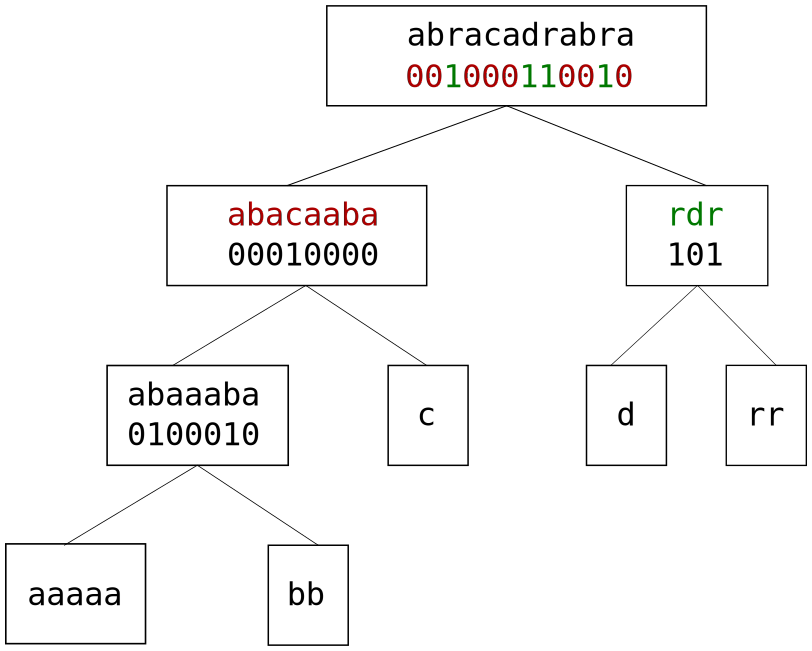
\includegraphics[width=0.9\textwidth]{WTdrawing.pdf}
\end{center}
}

\newpage
\tableofcontents
\newpage


\vspace*{\fill}
\begin{abstract}
In this thesis we perform a survey on the applications of wavelet trees.
We also implement various versions of wavelet trees, each version an attempt at improving the previous.
For each version we test and compare the running times of construction and queries on the wavelet tree. 
We analyse the results using Cache Miss, Branch Misprediction and Translation Lookaside Buffer Miss measurements to explain the differences in the running time, and as and inspiration for the next attempt at optimization.
From our analysis and tests we find various changes that improve the query running times on the wavelet tree, and also some that worsen the running time even when improving some of the other measurements.
\end{abstract}
\vspace*{\fill}
\newpage

\part{The Wavelet Tree}

\section{Introduction}
The Wavelet Tree is a relatively new data structure first introduced in 2003 by Grossi, Gupta, and Vitter~\cite{Grossi:2003:HET:644108.644250} that is built on a sequence of characters from an alphabet and supports rank and select queries on the sequence.
According to Gonzalo Navarro~\cite{Navjda13} and others[TODO: cite others] the wavelet tree has many and wide ranging useful applications, from string processing including full-text indexes and inverted indexes to geometry processing including point grids and rectangle sets as well as graphs.

In this thesis we wish to implement various algorithms and data structures for storing, constructing and querying a wavelet tree, test and compare their running times and memory usage and analyse the practical reasons for their running times and memory usage such as Cache Misses (CM), Branch Mispredictions (BM), and Translation Lookaside Buffer Misses (TLBM). Directly inspired by this analysis we will attempt a number of optimizations aimed at reducing these measurements.

We will first implement the basic construction algorithm based on the description found in~\citep{ Navjda13}.
We will then implement and attempt to improve the rank and select query algorithms.
We will also implement a more advanced algorithm constructing a \textit{wavelet suffix tree}, which is different, yet analogous, to a wavelet tree, but with a better theoretical running time, as described in~\citep{DBLP:journals/corr/BabenkoGKS14}. Finally, we will implement a parallelized version as described in~\citep{DBLP:journals/corr/Shun14}

Our focus will be to implement something useful in real world scenarios and we will use inputs we believe to be realistic use cases.
We will also avoid impractical optimizations such as ones that require recompilation to handle different sizes or alphabets.

\section{Related Work}
The wavelet tree was first introduced in 2003 by Grossi, Gupta, and Vitter~\cite[Section 4.2]{Grossi:2003:HET:644108.644250} as a way to obtain faster rank and select query times on compressed suffix arrays while maintaining empirical entropy compression.

Later, and Gonzalo Navarro~\cite{Navjda13} explains how the wavelet tree has many and wide ranging useful applications, from string processing including full-text indexes and inverted indexes to geometry processing including various queries and computations on point grids and rectangle sets as well as graphs.

Cristos Makris~\citep{WTSurvey} also describes several uses for a wavelet tree, including effective storage compression using various ways of encoding the bitmaps, such as using Run-length encoding (RLE) on the bitmaps and storing the Burrows-Wheeler transformation (BWT) of the input string, or using Huffman Coding to shape the tree.
The Burrows-Wheeler transformation was introduced by Burrows and Wheeler~\citep{BWToriginalArticle} in 1994.
Ferragina et al.~\citep{waveletTreeEntropy} describes in more detail how BWT can be used to reduce the problem of compressing higher-order entropy to a problem of compressing 0-order entropy, which the wavelet tree then can do using RLE.
Mäkinen and Navarro~\citep[Section~4]{FMcountOnBWT} invented the Huffman-shaped wavelet tree and describes in short the general principle of it without going into much detail.

Another use of a wavelet tree is answering Range Quantile queries as is described by Gagie et al.~\citep[Section 3]{RangeQuantileQueries}.

Claude and Navarro~\citep[Section~2.2]{Claude08practicalrankselect} gives a good description of how rank and select queries is performed on the wavelet tree in practice.

\section{The Wavelet Tree}
The Wavelet Tree is a binary balanced tree structure, that was invented by Grossi, Grupta and Vitter \citep{Grossi:2003:HET:644108.644250} in 2003. 
It has applications in many areas; from string processing to geometry, and can for instance be used to represent; a sequence of elements, a reordering of elements and a grid of points. 
When \citep{Grossi:2003:HET:644108.644250} invented the Wavelet Tree, it was a milestone in compressed full-text indexing even though it is mentioned very little in the paper.
\textbf{[TODO: The Idea behind it, as well as for rank and select]}

\subsection{Constructing the Wavelet Tree}
A Wavelet Tree stores a string by creating a bitmap that describes the string using the alphabet of the string. The alphabet is split in the middle and the symbols to the left gets bit value 0 and the symbols to the right gets bit value 1 so that there is a bit for each symbol in the string in the bitmap. 
The symbols of the string that has bit value 0 is concatenated in the order they have in the string and is added to the left sub-tree and the ones with bit value 1 is added to the right sub-tree. 

This process continues in each sub tree until we end up in the leaves where the string only consists of one unique symbol from the alphabet. 
An example of a Wavelet Tree can be seen in Figure \ref{fig:WaveletTreeExample}. 
We now go into more detail about how it all works as described by \citep{Navjda13}.

\vspace{0.5 cm}
\begin{mdframed}[nobreak, linecolor=lightgray]
\textbf{Definition 1:} String representation in a Wavelet Tree

Let $S[1,n] = S_1 S_2 ... S_n$ be a sequence of symbols where $s_i \in \Sigma$ and $\Sigma = [1 .. \sigma]$ is the alphabet. $S$ can then be represented in plain form using $n \lceil \log \sigma \rceil = n \log \sigma = O(n)$ bits.
\end{mdframed}
\vspace{0.5 cm}


\figureBegin
\caption{Wavelet Tree on string \textit{adsfadaadsfaads}}				
\Tree
%root
[.adsfadaadsfaads\\001100000110001 !\qsetw{5cm} 
	%left child
	[.adadaadaad\\0101001001 !\qsetw{5cm}
		%left -> left,right child 
		[.aaaaaa\\000000 !\qsetw{5cm} ] [.dddd\\1111 !\qsetw{5cm} ]] 
	%right child
	[.sfsfs\\10101 !\qsetw{5cm} 
		%right -> left,right child
		[.ff\\00 !\qsetw{5.3cm} ] [.sss\\111 !\qsetw{5.3cm} ]]] 
\vspace{1 cm}
\label{fig:WaveletTreeExample}
\figureEnd

		
A Wavelet Tree can be described recursively over a sub-alphabet range $[a .. b] \subseteq [1 .. 0]$, for a sequence $S[1,n]$ over alphabet $[1 .. \sigma]$. 
A Wavelet Tree over alphabet $[a .. b]$ is a binary balanced tree with $b - a + 1$ leaves. If $a = b$ then the Wavelet Tree is simply a leaf labelled a. 
Otherwise it has an internal root node $v_{root}$ that represents the string $S[1,n]$. 
\textproc{BitmapConstruction} (Algorithm~\ref{alg:BitmapConstruction}) describes how $v_{root}$ constructs bitmap $B_{v_{root}}$. $B_{v_{root}}$ is stored in $v_{root}$.

\begin{algorithm}
\caption{Construction of a bitmap from a string \textit{S}}
\label{alg:BitmapConstruction}
\begin{algorithmic}
\Function{BitmapConstruction}{$S$}
\If{ $S[i] \leq (a + b)/2$ }
	\State $B_{v_{root}}[i] \gets 0$
\Else
	\State $B_{v_{root}}[i] \gets 1$
\EndIf
\EndFunction
\end{algorithmic}
\end{algorithm}


Knowing how to construct the bitmap in the root of the Wavelet Tree we now define (Definition 2) how string is split in two and saved in the roots of right and left sub=trees which are also Wavelet Trees.


\vspace{0.5 cm}
\begin{mdframed}[nobreak]
\textbf{Definition 2:} Splitting the string. \\

\noindent
Let $S_0[1,n_0] =$ subsequence of $S[1,n]$ formed by symbols $c \leq (a + b)$/2.

\noindent
Let $S_1[1,n_1] =$ subsequence of $S[1,n]$ formed by symbols $c > (a + b)$/2.
\\ \linebreak
\noindent
Then the left child of $v_{root}$ is a Wavelet Tree for $S_0[1,n_0]$ over alphabet $[a .. \lfloor (a + b)/2 \rfloor]$ and right child of $v_{root}$ is a Wavelet Tree for $S_1[1,n_1]$ over alphabet $[1 + \lfloor (a + b)/2 \rfloor .. b]$. 
\end{mdframed}
\vspace{0.5 cm}

Having generated the left and right sub-trees the construction process (splitting of string and bitmap construction) continues recursively on the root of each of the sub-trees until it end up in a leaf.

\subsubsection{Complexity}
The height of the Wavelet Tree is  $\lceil \log \sigma \rceil$ and it has $\sigma$ leaves and $\sigma - 1$ internal nodes. 
At each level in the tree n bits are stored and in the last level at most n bits are stored. $n \lceil \log \sigma \rceil$ is an upper bound to the total number of bits that the Wavelet Tree stores. 
The Wavelet Tree can be constructed in $O(n \log \sigma)$ time.

\subsection{Rank Query}
Rank counts the number of occurrences of the specified character up to and including the specified position. 
It starts from the root of the Wavelet Tree and moves down through the tree until it hits the leaf of the input character, \citep[Section 2.2]{Claude08practicalrankselect}.

\begin{algorithm}
\caption{Rank}
\label{alg:rank}
\begin{algorithmic} 
\Function {Rank} {$Character, Position$}
\If{$Self.IsLeaf()$}
\State \Return $Position$
\EndIf
\State $CharBit \gets$ bit representing $Character$ in bitmap of current node
\State $Position \gets$ \Call {BinaryRank} {$CharBit, Position, BitMap$}
\If{$CharBit = 1$}
	\State $Rank \gets$ RightChildNode.\Call {Rank} {$CharBit, Position$}
\Else
	\State $Rank \gets$ LeftChildNode.\Call {Rank} {$CharBit, Position$}
\EndIf
\State \Return $Rank$ 
\EndFunction
\State RootNode.\Call {Rank} {$Character, Position$}
\end{algorithmic}
\end{algorithm}


\noindent \textproc{Rank($Character, Position$)} in our implementation is defined on each node, which is why it is called on the root node and the right and left child nodes in stead of specifying the node as a parameter to the \textproc{Rank} function, here in the pseudo-code.

\subsubsection{Binary Rank} 
\label{sec:TheoryBinaryRank}
A cornerstone of the rank algorithm for a Wavelet Tree is calculating the binary rank of a character on a bitmap at a node.
The naive implementation of \textproc{BinaryRank} where you loop through the binary number and count the number of 1s or 0s takes O(N) time, which is too much because the running time of the rank algorithm depends on the running time of \textproc{BinaryRank} since \textproc{BinaryRank} is called once per layer of the tree in order to answer a single rank query on the tree.

To make binary rank fast, we later used the \texttt{popcount} instruction that counts the number of 1s in the binary represenation of a given number. See section~\ref{sec:popcountBinaryRank}.

\subsection{Select query}
\textproc{Select} queries the Wavelet Tree for the position of the i'th occurrence of the specified character.
It starts from the leaf of the character and queries up through the tree, which means you need to know the leaf of the character in advance \citep[Section 2.2]{Claude08practicalrankselect}. 


\begin{algorithm}
\caption{Select}
\label{alg:select}
\begin{algorithmic} 
\Function {Select} {$Character, Occurrence$}
\If{$CurrentNode$ is $RightChild$}
	\State $CharBit \gets 1$
\Else
	\State $CharBit \gets 0$
\EndIf
\State \Return $Parent.$\textproc{SelectRec}$(CharBit, Occurrence)$
\EndFunction

\vspace{1cm}

\Function {SelectRec} {$CharBit, Occurrence$}
\If{$CurrentNode$ is $root$}
	\State \Return \textproc{BinarySelect}$(CharBit, Occurrence)$
\EndIf
\State $Position \gets $\textproc{BinarySelect}$(CharBit, Occurrence)$
\If{$CurrentNode$ is $RightChild$}
	\State $CharBit \gets 1$
\Else
	\State $CharBit \gets 0$
\EndIf
\State \Return $Parent.$\textproc{SelectRec}$(CharBit, Position)$
\EndFunction
\end{algorithmic}
\end{algorithm}


We split Select into two functions; \textproc{Select} which is called on the leaf and \textproc{SelectRec} which is called from \textproc{Select} on the parent of the leaf and continues recursively until the root is reached. 
This makes sense because it saves us a check for whether we are a leaf or not at each recursive call and since we start out in a leaf and will never meet one again that check would only be true once. 

Figuring out the \textproc{CharBit} is a lot easier for \textproc{Select} than for \textproc{Rank} since we query bottom-up and can just check whether the current node is a left child or a right child. 
In \textproc{Rank} one needs to calculate the split character and then check whether the input character is before or after it in the alphabet.

\subsubsection{Binary Select}
\textproc{BinarySelect} returns the position of the i'th occurrence of 1 or 0 (\textproc{CharBit}) in a bitset. 
The simple implementation is to loop through the bitset and when $i$ occurrences of either 1 or 0 has been seen then return the position of the last one. 
This takes O(N) time making \textproc{BinarySelect} a huge bottleneck for \textproc{Select} since it is called for each level in the Wavelet Tree. 
In \ref{sec:ImplBinarySelect} we describe how to improve the practical running time of \textproc{BinarySelect} using the \textit{popcount} instruction.

\subsection{Applications}
\subsubsection{Compression}
The Wavelet Tree is used for compression of data in a lot of ways where two of the main techniques are using specific encodings on bitmaps and changing the shape of the tree \citep[Section~3]{Navjda13}.
The type of encoding on bitmaps that is used most often is entropy coding.

Entropy coding can be explained by splitting it into two parts: Modelling and Coding.
Modelling assigns probabilities to the symbols of the string, and coding produces a bit sequence from these probabilities.
The probability of a symbol is based on how often it appears in a given data set. 
Higher frequency gives a higher probability.
Entropy coding can be done with a coding scheme, which uses a discrete number of bits for each symbol, for example Huffman coding. 
Entropy can be defined as:

\begin{mdframed}[nobreak, linecolor=lightgray]
\textbf{Definition}: Entropy. \\
Let \textit{S} be a sequence of \textit{n} symbols from an alphabet $\Sigma = \lbrace c_1 ... c_\sigma \rbrace$ of cardinality $\sigma$.
Then \textit{entropy} H is defined as
\begin{center}
$H = \sum_{i=1}^{\sigma} p_i log_2(\frac{1}{p_i})$
\end{center}
where $p_i$ is the probability of the i-th symbol in the alphabet appearing in \textit{S}. 
\end{mdframed}

Entropy represents a lower bound to the average numbers of bits needed to represent each symbol in S, according to the coding theorem of Shannon (todo reference) and so is a useful value to compare with when trying to achieve good compression.

But this theoretical definition of entropy is often replaced in scientific literature by a more practical definition: \textit{empirical entropy}.
There are two versions: \textit{empirical zero-order entropy} $H_0$ and \textit{empirical k-th order entropy} $H_k$. $H_k$ takes the size \textit{k} context of the symbol appearances into account while $H_0$ does not and treats symbols independently instead. 

\begin{mdframed}[nobreak, linecolor=lightgray]
\textbf{Definition}: \textit{Empirical zero-order entropy}, $H_0$ \\
Let \textit{S} be a sequence of \textit{n} symbols from an alphabet $\Sigma = \lbrace c_1 ... c_\sigma \rbrace$ of cardinality $\sigma$.
Then \textit{entropy} $H_0$ is defined as
\begin{center}
$H_0 = \sum\limits_{c_i \in \Sigma} \frac{n_i}{n} log_2(\frac{n}{n_i})$
\end{center}
where $n_i$ is the number of appearances of character $c_i$ in $S$.
\end{mdframed}

\begin{mdframed}[nobreak, linecolor=lightgray]
\textbf{Definition}: \textit{Empirical k-th order entropy}, $H_k$ \\
For a string $w \in \Sigma^k$ let us denote with $w_S$ the subsequence of characters that follow \textit{w} in \textit{S}, then the k-th order empirical entropy of \textit{S}, is defined as follows:
\begin{center}
$H_k(S) = \frac{1}{n} \sum\limits_{w \in \Sigma^k} | w_S |H_0(w_S)$
\end{center}
\end{mdframed}

The wavelet tree can be used to both achieve space within \textit{zero-order entropy} and \textit{k-th order entropy}. To achieve \textit{zero-order entropy} a Huffman shaped wavelet tree (todo: reference) can be used. But when the alphabet is very large that is not a good approach with regards to compression, because storing the huffman symbol assignments and wavelet tree pointers ends up using too much space . \citep[Section~3]{Claude08practicalrankselect} describes a way to also have \textit{zero-order entropy} space usage for large alphabets. 








\section{Applications}
\subsection{What The Wavelet Tree Can Represent}
\textbf{[TODO: redo this subsection]}
The Wavelet Tree has multiple applications that each utilize the wavelet tree differently and use it for storage of, and queries on, different types of data.
These can be split into three main types: A sequence of values, a reordering or permutation, and a grid of points.

Using the Wavelet Tree to store a sequence of values is perhaps the most basic way to utilize the tree.
The Wavelet Tree stores the values and their sequence and supports access, rank, and select queries.

The Wavelet Tree can also be used to describe a stable reordering, e.g. of the symbols in a string S. 
If the leaves are traversed then all the occurrences of the smaller symbols are found first. \textbf{[TODO: describe the use of traversing the leaves like so]}
By tracking the position of a symbol downwards through the Wavelet Tree we will find the new position of the symbol after the permutation.
Tracking the position of a symbol upwards through the wavelet tree will where it is in the original string. 

A Wavelet Tree can also represent a $n \times n$ grid of $n$ points where no two points share the same row or column. 
One can map a general set of $n$ points to such a discrete grid and then store the real points somewhere else.

If we have points sorted by the $x$-coordinate and take only the $y$-coordinates $S_y[1,n] = y_1,y_2,...,y_n$ and save $S_y$ in a Wavelet Tree we can the find the \textit{i}th point in $x$-coordinate order by accessing the corresponding $y$-coordinate in the wavelet tree. 
If we want the \textit{i}th point in $y$-coordinate order we can access the leaf of a given $y$-coordinate and find its corresponding $x$-coordinate by querying up through the tree until we find the original position of $y$ in $S$. 
The corresponding $x$-coordinate will be at the same position.
Querying from a leaf gives the points in $y$-coordinate order because the leaves are sorted by $y$-coordinate.

\subsection{Compression}
\vspace{0.5 cm}
\begin{mdframed}[nobreak, linecolor=lightgray, linewidth=2pt]
\begin{definition}: String representation in a Wavelet Tree\\\\
Let $S[1,n] = S_1 S_2 ... S_n$ be a sequence of symbols where $s_i \in \Sigma$ and $\Sigma = [1 .. \sigma]$ is the alphabet. $S$ can then be represented in plain form using $n \lceil \log \sigma \rceil = n \log \sigma = O(n)$ bits.
\end{definition}
\textbf{[TODO: use and reference this]}
\end{mdframed}
\vspace{0.5 cm}
The Wavelet Tree has many uses for compression of data~\citep{Navjda13}. Some of the main compression techniques are different ways of encoding the bitmaps and changing the shape of the tree \citep[Section~3]{Navjda13}.

\textbf{[TODO: either move or remove this paragraph]}
Entropy coding can be explained in two parts: Modelling and Coding.
Modelling assigns probabilities to the symbols of the string, and coding produces a bit sequence from these probabilities.
The probability of a symbol is based on how often it appears in a given data set. 
Higher frequency gives a higher probability.
Coding can then for instance be done with a coding scheme, that uses a discrete number of bits for each symbol, for example Huffman Coding \citep{HuffmanCoding}.

The main advantage of the wavelet tree with regards to compression is that it supports entropy bounds in the attained space complexity of the various wavelet tree compression methods \citep[Section~2.1]{WTSurvey}.

\subsubsection{Entropy}
According to \citep[Introduction]{WTSurvey} entropy can be defined as:

\begin{mdframed}[nobreak, linecolor=lightgray, linewidth=2pt]
\begin{definition}: Entropy \\\\
Let \textit{S} be a sequence of \textit{n} symbols from an alphabet $\Sigma = \lbrace c_1 ... c_\sigma \rbrace$ with cardinality $\sigma$.
Then \textit{entropy} H is defined as
\begin{center}
$H = \sum_{i=1}^{\sigma} p_i log_2(\frac{1}{p_i})$
\end{center}
where $p_i$ is the probability of the i-th symbol in the alphabet appearing in \textit{S}.
\end{definition} 
\end{mdframed}

Entropy represents a lower bound to the average number of bits needed to represent each symbol in $S$ according to the coding theorem of Shannon~\citep[Introduction]{WTSurvey} and is the bound that compression researchers compare their results to.

This theoretical definition of entropy is often replaced in scientific literature by a more practical definition: \textit{empirical entropy}.
There are two versions: \textit{empirical zero-order entropy} $H_0$ and \textit{empirical k-th order entropy} $H_k$. $H_k$ takes into account a context of size \textit{k} of the symbol appearances, ie. the suffixes of length $k$ of each symbol appearance in the string, while $H_0$ does not and treats symbols independently instead. 

\begin{mdframed}[nobreak, linecolor=lightgray, linewidth=2pt]
\begin{definition}: \textit{Empirical zero-order entropy}, $H_0$ \\
Let \textit{S} be a sequence of \textit{n} symbols from an alphabet $\Sigma = \lbrace c_1 ... c_\sigma \rbrace$.
Then \textit{entropy} $H_0$ is defined as
\begin{center}
$H_0 = H_0(S) = \sum\limits_{c_i \in \Sigma} \frac{n_i}{n} log_2(\frac{n}{n_i})$
\end{center}
where $n_i$ is the number of appearances of character $c_i$ in $S$.
\end{definition}
\begin{definition}: \textit{Empirical k-th order entropy}, $H_k$ \\
For a string $w \in \Sigma^k$ let us define $w_S$ as the concatenation of characters that follow \textit{w} in \textit{S}. 
Then the k-th order empirical entropy of \textit{S}, is defined as follows
\begin{center}
$H_k = H_k(S) = \frac{1}{n} \sum\limits_{w \in \Sigma^k} | w_S |H_0(w_S)$
\end{center}
\end{definition}
\end{mdframed}
$H_k$ often defines a lower bound for bit space usage that is smaller than the lower bound of $H_0$\citep[Section~2]{waveletTreeEntropy}.

Using the Burrows-Wheeler transformation on the input the we can reduce the problem of achieving $H_k$ compression to achieving $H_0$ compression.
In other words, if we have a good compression algorithm that achieves compression within the $H_0$ lower bound, then by using that algorithm on the Burrows-Wheeler transformation of the input we can achieve compression within the $H_k$ lower bound~\citep[Introduction]{waveletTreeEntropy}.
The problem for a long time was that there existed no good way to achieve compression within the $H_0$ lower bound or at least it was a problem before the wavelet tree was invented~\citep[Introduction]{waveletTreeEntropy}.

To achieve \textit{zero-order entropy} a Huffman shaped wavelet tree can be used~\citep[Section~4]{FMcountOnBWT}. Claude and Navarro~\citep[Section~3]{Claude08practicalrankselect} describes a way to also have \textit{zero-order entropy} space usage for large alphabets. 
It is therefore possible to get space usage within \textit{zero-order entropy} even for large alphabets using the wavelet tree. 
\textit{Zero-order entropy} can also be achieved by run-length encoding the bitmaps in the wavelet tree, which is also the approach that is used when compressing the \textit{bwt} transformation of the input string using the wavelet tree \citep[Introduction (\textbf{B})]{waveletTreeEntropy}.
This means that using a combination of run-length encoding of bitmaps and taking the Burrows-Wheeler transformation of the input string using the wavelet tree it is possible to achieve compression near the lower bound of \textit{k-th order entropy}.

\subsubsection{Run-Length encoding}
Run-length encoding (RLE) is a simple process where the number of consecutive repeats of each symbol is stored in stead of storing the symbols them selves. 
If we have the string \textit{aaaaacccaaaaabbbaa} we can run-length encode this to \textit{a5c3a5b3a2} which is a smaller string containing the same information.
It is necessary to store the symbol and it's number of consecutive repeating occurrences because we need to be able to identify which symbol occurs where and how many times in order to be able to reproduce the original string.
The longer the sequence of a repeating symbol is the less space is used, since it can be stored as one number plus the related symbol.

When representing the string using a wavelet tree, the problem gets reduced to run-length encoding a string of bits (the bitmap in each node).
Since a binary number only has an alphabet with the cardinality of two we do not need to store both the symbol and its occurrence but only the occurrence.
If we define that the first number is always the amount of 0s and the second number is always the amount of 1s and so forth. 
Then by looking at the bitmap of \textit{aaaaacccaaaaabbbaa} which is \textit{000001110000000000} when stored in a wavelet tree we can encode it into $(5,3,10)$.
Figure~\ref{fig:RleWaveletTree} shows an example of a wavelet tree with run-length encoded bitmaps.

If we do not consider how a computer saves numbers but only consider the amount of numbers that needs to be stored then $RLE(000001110000000000)$ achieves a great reduction in space.
From 18 numbers to only 3 numbers, which contain the same information.

If we do consider how a computer saves numbers then the reduction is not that great because if we assume that each number is represented as an integer, then the run-length encoded bitmap uses more space than just storing the original bitmap. 
This is because an integer uses 4 bytes of space which is 32 bits and we need to store three integers giving us a total of $32 bits \times 3 = 96 bits$ which is significantly larger than just the 18 bits we need to store for the original bitmap assuming we can store 1 and 0 using only 1 bit \footnote{This can be accomplished using C++ and Vector$<$bool$>$}. 
This means that the symbols in the string need to, on average, repeat consecutively more than 32 times before RLE achieves better space usage than just storing the bitmaps.

RLE is still very useful despite of this because you usually want to compress very large data and if that data uses an alphabet that is small enough then, as previously stated RLE can achieve compression close to the \textit{zero order entropy} when working with binary alphabets.

If the Burrows-Wheeler transformation is applied to the string before it is saved in the wavelet tree and run-length encoded then the number of consecutive repeats of a symbol is increased which enables even greater compression.

\subsubsection{Burrows-Wheeler transformation}
Having a string \textit{S} of \textit{n} characters the Burrows-Wheeler transformation \citep{BWToriginalArticle} transforms \textit{S} by forming \textit{n} cyclic shifts of \textit{S}. 
These \textit{n} permutations of \textit{S} are then sorted in lexicographical order.
The \# is added to keep track of the end of the original string.
The \textit{bwt} of \textit{S} is then the concatenation of the last characters in each permutation excluding $\#$.

\begin{center}
$\begin{bmatrix}
	bananahat\#\\
	ananahat\#b\\
	nanahat\#ba\\
	anahat\#ban\\
	nahat\#bana\\
	ahat\#banan\\
	hat\#banana\\
	at\#bananah\\
	t\#bananaha\\
	\#bananahat\\
\end{bmatrix} \Rightarrow
\begin{bmatrix}
	\#bananaha\textbf{t}\\
	ahat\#bana\textbf{n}\\
	anahat\#ba\textbf{n}\\
	ananahat\#\textbf{b}\\
	at\#banana\textbf{h}\\
	bananahat\#\\
	hat\#banan\textbf{a}\\
	nahat\#ban\textbf{a}\\
	nanahat\#b\textbf{a}\\
	t\#bananah\textbf{a}
\end{bmatrix}$
\end{center}

The list to the left is the permuted versions of \textit{S} and the list to the right is the lexicographically sorted permutations of \textit{S}.
Taking the character at the last index in each column the Burrows-Wheeler transformation of $S=bananahat$ becomes $bwt(S) = tnnbhaaaa$. The index of the the original string in the right list is also returned. 
The original string is identified by having a \# at the end.

Looking at \textit{bwt(S)} we can see that equal characters are now grouped together.
This effect enables better compression when using compression techniques like run-length encoding.
One could argue that simply sorting \textit{S} would enable better compression using run-length encoding, which is true, but a sorted sequence is not reversible, which BWT is.
It would not make very much sense to compress something without being able to decompress it again.
Burrows et al.~\citep[Section~2]{BWToriginalArticle} describes an algorithm for getting the original string from the Burrows-Wheeler transformed string.

Figure~\ref{fig:BwtRleWaveletTree} depicts a RLE Wavelet tree on \textit{bwt(abcbadbd)}. We can see, as indicated by the numbers in bold that fewer Run-length encoded values needs to be stored than for the non-Burrows-Wheeler transformed case as shown in figure~\ref{fig:RleWaveletTree}.
\figureBegin
      \begin{minipage}{0.45\textwidth}      
			\Tree
			%root
			[.bananahat\\2,1,1,1,3,1 !\qsetw{3cm} 
				%left child
				[.baaaha\\1,2,1,1 !\qsetw{3cm}
					[.baaaa\\0,1,4 !\qsetw{3cm}
						[.aaaa !\qsetw{3cm} ]
						[.b !\qsetw{3cm} ]		
					] 
					[.h !\qsetw{3cm} ]
				] 
				%right child
				[.nnt\\2,1 !\qsetw{3cm}	
					[.nn !\qsetw{3cm} ] 
					[.t !\qsetw{3cm} ]
				]
			]
		\caption{RLE Wavelet Tree on string \textit{bananahat} with alphabet $\sigma = abhnt$}
      \label{fig:RleWaveletTree}
	\end{minipage}
	\hfill
	\begin{minipage}{0.45\textwidth}	
			\Tree
			%root
			[.tnnbhaaaa\\\textbf{0,3,6} !\qsetw{3cm} 
				%left child
				[.bhaaaa\\\textbf{1,1,4} !\qsetw{3cm} 
					[.baaaa\\0,1,4 !\qsetw{3cm} 
						[.aaaa !\qsetw{3cm} ]
						[.b !\qsetw{3cm} ]		
					] 
					[.h !\qsetw{3cm} ]
				] 
				%right child
				[.tnn\\0,1,2 !\qsetw{3cm}		
					[.nn !\qsetw{3cm} ] 
					[.t !\qsetw{3cm} ]
				]
			] 
		\caption{RLE Wavelet Tree on $BWT(bananahat)=tnnbhaaaa$ with alphabet $\sigma = abhnt$}
		\label{fig:BwtRleWaveletTree}
	\end{minipage}
\figureEnd

One might wonder how \textproc{Rank} and \textproc{Select} queries can be useful when the string is Burrows-Wheeler transformed and therefore permuted resulting in the queries values that is essentially unrelated to the original string \textit{S}. 

The queries does have uses when working with the \textit{FM-index}, named after its inventors Paolo Ferragina and Giovanni Manzini, which is a self-index based on the Burrows-Wheeler transformation $BWT(S)$ that is able to find occurrences and positions of patterns (sub-strings) in \textit{S} by looking at $BWT(S)$. 
Such a procedure is described in \citep[Section 2]{FMcountOnBWT}.

\subsubsection{Huffman-shaped Wavelet Trees}
\citep[Section~4]{FMcountOnBWT} describes a Huffman Shaped Wavelet Tree which places symbols with higher frequencies closer to the root than those that have a lower frequency, in such a way that the path from root to symbol leaf corresponds to the binary Huffman code of the symbol. Using a Huffman Shaped Wavelet Tree is an alternative to run-length encoding.
The Huffman code of a symbol is a small binary value for symbols with high frequency and a larger binary value for symbols with the small frequency.
This approach would make the tree skewed and as a result increase the height of the tree but decrease query time for symbols with high frequency.
If one then queries the Huffman shaped Wavelet Tree for a symbol that has a high frequency then one would find it faster than if one was looking for a symbol that was less frequent.

Since the Huffman encoding is based on frequency of symbols it achieves the best performance and space complexity when symbols are non-uniformly distributed.
If the data is uniformly distributed then the length of all Huffman codes would be similar resulting in a balanced tree having performance and space complexity similar to a normal Wavelet Tree.
Since we have primarily used uniformly distributed data in our experiments, and because of limited time, we have not implemented and done experiments on a Huffman Shaped Wavelet Tree.
In section~\ref{sec:choiceOfInputString} we discuss why we mainly consider uniform data.


\subsection{Information Retrieval}
\textbf{[Perhaps TODO: Wavelet tree as a Range Searching Data Structure]}


\subsubsection{Range Quantile Query}
A range quantile query is a query that returns the $k$th smallest number within a subrange of a given sequence of elements.
So if we are e.g. given a list of price changes on a laptop during the last year then a range quantile query is able to answer what the smallest or third smallest (indicated by the k value) price of the laptop was within for instance a month of that year.
It is therefore also quite easy to find quantiles like the 2-quantile (median) or the 3-quantile. 
To e.g. find the median, $k$ can be defined as half the length of the range of the sequence.
This would return the middle element of the subsequence.
The 3-Quantile can be found by setting $k$ to $\frac{1}{3}$ of the length of the subsequence. 
Quantiles are important values and are used a lot in statistics.

The wavelet tree can be used to support efficient range quantile queries on a sequence \textit{S} of \textit{n} numbers in $O(\log(\sigma))$ time if $rank_b$ is supported in $O(1)$ time \citep[Section 3]{RangeQuantileQueryWT}. 
The range is denoted as $S[l ... r]$.
A range quantile query based on a wavelet tree works by computing two rank queries on the bitmap of each node in a traversal from the root to a leaf node. 

\begin{algorithm}
\caption{Range Quantile Query}
\label{alg:RangeQuantileQuery}
\begin{algorithmic}
\Function {RangeQuantileQuery} {$k,l,r$}
\If{current node is leaf}
	\State \Return number in leaf
\EndIf
\State $\textit{0}sInRange \gets rank_0(S \lbrace l..r \rbrace) = rank_0(r) - rank_0(l-1)$
\If{$\textit{0}sInRange \leq k$}
	\State $l = rank_0(l-1))+1$
	\State $r = rank_0(r)$
	\State \Return $LeftNode.RangeQuantileQuery(k,l,r)$
\Else
	\State $k = k - \textit{0}sInRange)$
	\State $l = rank_1(l-1)+1$
	\State $r = rank_1(r)$
	\State \Return $RightNode.RangeQuantileQuery(k,l,r)$
\EndIf

\EndFunction
\end{algorithmic}
\end{algorithm}

The two queries are $rank_b(l-1)$ and $rank_b(r)$ where $rank_b$ is the binary rank.
$rank_b(l-1)$ is used to find the number of 1s and 0s in $b[1..(l-1)]$ and $rank_b(r) - rank_b(l-1)$ gives the number 1s and 0s in $b[l..r]$. 
We go to the left if there are more than \textit{k} 0s in $b[l..r]$ and set $l = ($number of 0s in $b[1..(l-1)])+1$ and $r=($number of 0s in $b[1..r])$. 
We go to the right if there are less than \textit{k} 0s in $b[l..r]$ and subtract the number of 0s in $b[l..r]$ from \textit{k} and set $l = ($number of 1s in $b[1..(l-1)])+1$ and set $r=($number of 1s in $b[1..r])$. 
This procedure continues recursively until it hits a leaf and then returns the number stored in the leaf which corresponds to the $k$th smallest number in $S[l..r]$.

Algorithm~\ref{alg:RangeQuantileQuery} describes the pseudo-code for a range quantile query where $rank_1$ is a binary rank query which returns the number of 1s in the bitmap of $S$ in each node generated by the wavelet tree. 
$rank_0$ return the number of 0s.
The argument to $rank_0$ and $rank_1$ is the position to find the number of occurrences up to.
This means that $rank_1(r)$ for instance returns the number of 1s in the bitmap until position $r$.

\figureBegin
\begin{minipage}{.45\linewidth}
\begin{flushleft}                           
\Tree
%root
[.6,2,\textbf{0,7,9,3,1,8,5},4\\1001100110 !\qsetw{5cm} 
	%left child
	[.2,0,3,1,4\\00101  !\qsetw{5cm}
		%left -> left
		[.2,0,1\\100 !\qsetw{5cm} 
			[.0,1\\01 
				[.0 ]
				[.1 ] 			
			]
			[.2 ]		
		] 
		%left -> right
		[.3,4\\01 !\qsetw{5cm} 
			[.3 ]
			[.4 ]		
		]
	] 
	%right child
	[.6-\textbf{7,9,8,5}\\00110 !\qsetw{5cm} 
		%right -> left
		[.6,\textbf{7,5}\\010 !\qsetw{5.3cm}
			%right -> left -> left
			[.6,5\\10 
				[.5 ]
				[.6 ]			
			] 
			%right -> left -> right
			[.\textbf{7} ] 
		]
		%right -> right	 
		[.9,8\\10 !\qsetw{5.3cm} 
			[.8 ]
			[.9 ]		
		]
	]
] 
\end{flushleft} 
\end{minipage}
\hfill
\begin{minipage}{.45\linewidth}
\begin{flushright}
Level 1:\\$k=5$\\$l=3$\\$r=9$\\ \vspace{0.5cm}
Level 2:\\$k=2$\\$l=2$\\$r=5$\\ \vspace{0.5cm}
level 3:\\$k=2$\\$l=2$\\$r=3$\\ \vspace{0.5cm}
Level 4:\\$k=1$\\$l=1$\\$r=1$
\end{flushright} 
\end{minipage}
\caption{Range Quantile Query on a Wavelet Tree. $S=\lbrace 6,2,0,7,9,3,1,8,5,4 \rbrace, k=5, l=3, r=9$.}
\label{fig:RQQWaveletTree}
\figureEnd

An example of a range quantile query can be seen in figure~\ref{fig:RQQWaveletTree}. 
The numbers in bold indicates the range $S[l..r]$ where $S= \lbrace 6,2,0,7,9,3,1,8,5,4 \rbrace$ and $l=3$, $r=9$ and $k=5$.
$k=5$ means that we are looking for the 5th smallest number within $S[l..r]$ which is \textit{7} indicated by the leaf that the query ends up in before terminating.
$l$ and $r$ indicates the range to look within.
The right side of the figure shows how \textit{k, l} and \textit{r} develops in each recursive call of the Range Quantile Query.

\newpage
\clearpage
\part{Hardware, Implementation \& Test}
In this part of the thesis we describe what hardware penalties we focus on optimizing and how and why they occur. 
We discuss choices we have made in the implementation like which C++ data structures to use. 
We also describe our test setup, what tools we have used for testing and discuss the effect of using uniform vs. non-uniform distributed data in our tests.

\section{Cache, Branch prediction and Translation Lookaside Buffer}

\subsection{Cache design and cache misses}

A cache is a small fast memory storage that holds the most recently used memory words.
Caches improves on the memory latency so memory access can be achieved within the demand of modern processors.
Modern memory systems usually have three caches: Level 1 (L1), Level 2 (L2) and Level 3 (L3). 

\begin{figure}
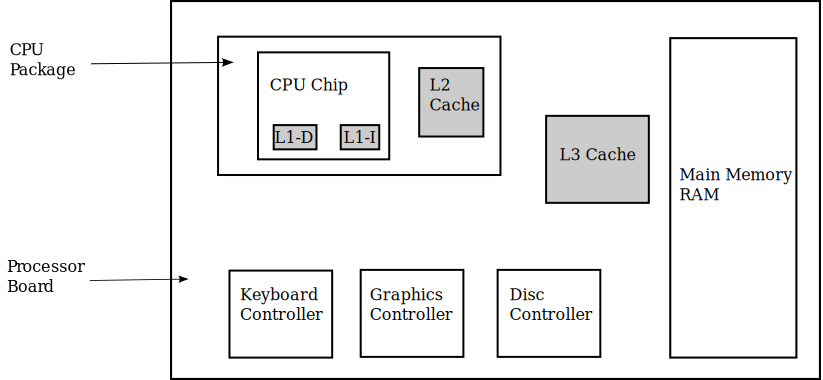
\includegraphics[width=\textwidth]{CacheLevels.pdf}
\caption{The three cache levels}
\label{fig:CacheLevels}
\end{figure}

Figure~\ref{fig:CacheLevels} shows how the three cache are placed in the relation to the CPU. 
The L1 cache resides on the CPU chip itself and usually has a size in the range from 16 KB to 128 KB and because it is placed directly on the CPU chip it is able to provide very fast memory access.
The L2 cache is placed next to the CPU chip on the CPU package and it is connected to the CPU via a high speed path. The L2 cache typically has a size between 512 KB and 1 MB which means that it can hold more data but is not able to provide as fast access as L1.
The L3 cache is placed on the processor board and usually has a size around 3 MB. Since it is placed further away from the cpu it is not able to provide as fast access as L1 and L2 but still much faster than fetching data from RAM.

All three caches are inclusive which means that L2 contains the data from L1 and L3 contains the data from L2.
This means that if data is evicted from L1 it will still reside in the L2 and L3 caches or if data is evicted from L2 it will still reside in L3. 
This is an advantage because it allows fast access to data even if it is evicted from L1 or L2. 
If the caches were not inclusive then it would result in a many more data requests to the main memory which is quite slow in relation to cache data access.

There are two types of address locality that the L1, L2 and L3 caches depends on; Spatial locality and Temporal locality.
Spatial locality occurs when memory locations that has addresses numerically similar to a recently accessed memory location are likely to be requested again very soon.
Temporal locality happens when memory locations that has been accessed recently are accessed again.
The cache exploits spatial locality by fetching more data than has been requested, assuming that it is possible to anticipate future requests.
Temporal locality is exploited by choosing what to evict on a cache miss and normally it is the data entries that has not been accessed recently that are evicted.

Data in the main memory is split into blocks of fixed size called \textit{cache-lines}. 
There are usually 4 to 64 consecutive bytes in a \textit{cache-line}. 
Some of these \textit{cache-lines} are always present in the caches. 
If a requested word is in the cache a trip to main memory can be saved but if the word is not in the cache then a \textit{cache-line} must be removed from the cache and the \textit{cache-line} containing the word must be fetched from main memory or a lower level cache if one is present. 
This is called a \textbf{cache miss} and has a high penalty because fetching a new \textit{cache-line} is expensive.
The general idea is to have the most heavily used \textit{cache-lines} in the caches as often as possible to reduce the amount of cache misses.

\subsubsection{Cache associativity}
When designing a cache it is important to consider whether each \textit{cache-line} can be stored in any cache slot or only in some of them.
There are three approaches to solving this problem; \textit{direct mapped cache}, \textit{n-way set-associative cache} and \textit{fully associative cache}. 
In a \textit{direct mapped cache} each \textit{cache-line} can only be stored in a specific cache slot.
This means that two \textit{cache-lines} cannot be mapped to the same slot simultaneously.
Given a memory address it is only necessary to look for it in one place in the cache and if it is not there then it is not in the cache. Using this approach post consecutive memory lines in consecutive cache slots. 




\subsection{Branch Mispredictions}

\subsection{Translation Lookaside Buffer misses}


\section{Notes on Implementation}

\subsection{Using Integers}
The Wavelet Tree is a data structure for strings of various size alphabets. Using the C++ \texttt{char array} or C++11 \texttt{string} types would seem natural in this case, but they each have problems.
The C and C++ \texttt{char} type is only of size 1 byte allowing us only to use an alphabet size of up to 256, making testing the running times dependency on alphabet size near-impossible.
The C++11 \texttt{string} and arrays of type \texttt{char32\_t} doesn't have this problem and supports character types up to 32-bit unsigned. The problem lies in output and readability as characters corresponding to byte values below 32 are special non-printable control characters such as carriage-return and backspace. At higher byte values other non-printable control characters and otherwise unreadable characters appear again, meaning we would have to be very selective with the allowed byte values in our alphabets if we want it to be readable for output and debugging, and likely end up with a non-continuous alphabet as a result.
Because of this, we have chosen to simply use arrays of integers as our strings in our implementations. Both characters and integers are simply different representations of byte values, so it will have no impact on performance or algorithm structure.

\section{Notes on The Experiments}
Here we discuss some things general for all our experiments, or all those where applicable.

\subsection{General Setup}
\label{sec:ExpNotesGeneralSetup}
We run 1000 queries 5 times for each variable parameter and register the total running time for each set of 1000 queries and then use the average of those 5 as the result.
Examples of variable parameters used in our tests are the alphabet size, the skew of the tree or the block size.

We calculate the standard deviation of the 5 runs and include that in the graphs as errorbars.
All our graphs with lines (as opposed to bar-graphs) include the standard deviation as errorbars.
If one appears not to have any errorbars that means the standard deviation is just very small.

\subsection{Choice of Input String}
We have chosen to construct the input strings used in our experiments so that each character occurs with the same probability at each position.
This means the string has a uniform distribution of characters from the alphabet.
We have chosen to do so for several reasons, among them being that we believe it to be a realistic use case \textbf{[TODO: why?]}, as well as making the choice of character to query for in our experiments make less difference.
The even amount of occurrences of each character also means there will be little difference in size of bitmap among the nodes in a single layer of the tree.

\subsubsection{Uniform vs. Non-Uniform data}
Uniform data for a wavelet tree is a string with each character occurring with the same probability at each position and therefore with similar frequencies.
If the data is non-uniform it means that some symbols from the alphabet will appear with a significantly higher frequency than others.
If one knows the frequencies of all symbols in the alphabet, without needing it to be exact, then one can build a Huffman shaped Wavelet Tree and we believe it will beat out any balanced wavelet tree in terms of performance.
The frequencies can be found by a simple linear scan of the input string before building the tree.

We are more interested in the general case of being able to perform well on any input string and so we don't want to implement optimizations that require a specific character distribution in the input string.
Using non-uniform data for our testing with a general wavelet tree will also introduce bias into our results.
This is because the sizes of the bitmaps in each node in a given level of the tree would not be equal, as they would for uniform data.
When we query the tree and take a path with many large bitmaps it will take longer than a path with many small bitmaps.
Depending on which non-uniform distribution is used, some characters might not even appear at all in the input string, and querying for them would terminate early.
This is especially true for Select queries that find the leaf node corresponding to the character that was queried for and then spends most of the its time traversing up the tree looking for the position in the complete input string.
If the queried-for character didn't exist in the input string, a select query would terminate before even having gone down the full length of the tree, because the leaf node corresponding to the character doesn't exist.
Rank queries on the other hand would still take much the same time on non-occurring characters as on occurring characters, because they spend most of their time in the single downward traversal of the tree they perform, and still will perform for non-occurring characters as it is only near the end of this traversal that the character will be found to not occur.

Therefore having nun-uniform data would introduce a bias in our query tests based on the symbol we are querying for, one that would be difficult to avoid without introducing more bias by choosing exactly which characters to query for.

There is also the problem of choosing which occurrence to query for in the case of select, as the character should occur at least that many times.
When using uniform data we know that it is extremely unlikely for any character to occur less than some minimum number of times, because of their equal occurrence probability.

If we used non-uniform data we would also have the problem of choosing which non-uniform distribution we should use, and there are many to choose from.

\subsubsection{Non-uniform distribution choice}
The wavelet tree has applications within full text indexing which suggests that having a distribution based on how words are distributed with in a normal English text could be a good choice, because it would be a realistic use case. 
Zipf's Law describes such a distribution \citep[abstract]{ZipfsLawOnText} but it requires a distribution parameter $s$ that describes the frequency relation between each symbol, e.g. if the most frequent word has double the frequency of the 2nd most frequent word and this relation continues down the list of most frequent words, it is a Zipf's Law distribution with an $s$ parameter of 2.
We have not been able to find anyone describing which parameter value would produce a distribution most closely resembling real world English. 
We have searched through various articles to find an \textit{s} value representative of the English language, but it does not seem like there is a single good value as it depends a lot on the type of text, e.g. scientific journals vs. newspapers vs. books.
This is also a conclusion that \citep[abstract]{ZipfsLawOnText} arrives at.

It is possible to estimate \textit{s} for a given text but doing so then creates the problem of choosing a representative text to estimate \textit{s} from.
We tried using the word frequencies in the NGSL \citep{NGSL} wordlist which contain the 31,241 most used words in the English language and the frequency with which they appear, to estimate \textit{s}.
NGSL is based on data from the Cambridge English Corpus which is a multi-billion word collection of written, spoken and learner texts and is the largest of its kind.
This fact combined with the fact that NGSL is fairly new (2013) makes us believe that the frequencies in the NGSL wordlist are accurate enough for our purpose.

Estimating \textit{s} using NGSL gave us a value very close to 1 which only grows closer to 1 the more words we used from the list.
This is a problem because with an $s$ parameter of 1, a Zipf's Law distribution is uniform.
It also tells us that the English language, or at least the part that has been aggregated in NGSL, might not, in fact, be following the Zipf's Law very closely, as we would expect our calculations to converge towards some constant value $>1$.
Instead we use the data from the NGSL word list and generate our own non-uniform dataset from it based directly on the word frequencies found in the NGSL word list.
This way we end up with a more realistic non-uniform dataset than if we had used the Zipf's Law model since the data is based on real empirical data and we avoid the problem of choosing a good \textit{s} value.


\subsection{Choice of Query Parameters}
\label{sec:choiceOfQueryParameters}
It is important to ensure that we don't introduce a bias in our experiments on the rank and select query performances by our choice of query parameters.
As we have chosen to use a randomly generated input string with uniform distribution of characters for most of our tests, there should be little difference in the frequency of characters and little difference in query performance based on the exact choice of character.
There is, however a difference of where in the tree the node each character corresponds to, and we should make sure to use characters from various positions in the alphabet, to have the queries together traverse as much of the tree as possible.

For the rank queries there is also the position parameter, determining how far into the string the query should look and therefore how far into each bitmap the query should look.
A high value (close to the length of the string) might seem like a good idea to make the query go through most of the bitmaps, but we don't want to introduce a bias by using some constant high value, nor do we want to risk introducing a bias by only looking at high values for the position parameter.
Again we choose to use values from all parts of the range of valid values for the parameter.

We are also interested in avoiding introducing any bias by using only one type of combination of parameters.
If we had e.g. let both parameter values depend on the index of a single for-loop around the call to the query, we would have only tested low character values together with low position values as well as high character values together with high position values.

Instead we let one parameter ascend from valid low values to valid high values with even spacing to reach the highest valid value in the lastly performed query. Meanwhile, the other parameter increases more rapidly with wider spacing, and then wraps around before passing highest valid value to then start again at low values, with an offset to not repeat parameter values, doing so many times before the end.
This ensures we perform the queries for all combinations of high, medium and low parameter values in our experiments.


\subsection{Tools Used}
We have looked at and tested the capabilities of several profilers and tools for determining the number of cache misses, branch mispredictions and translation lookaside buffer misses.


\subsubsection{Tools}
We have used these tools to count cache misses, branch mispredictions, etc., measuring memory usage and finding hotspots in our code.
\begin{description}
\item[Perf]~\citeB{perftool} is a performance analysing tools primarily implemented in the Linux kernel, available from version 2.6.31.
It supports reading and reporting various counters from the \textit{hardware}, meaning it does not emulate the CPU or anything similar, as some other tools like Callgrind do.
It can profile the entire system or a specific process, but not subsections of a program.
\item[PAPI]~\citeB{PAPI}, short for Performance Application Programming Interface, will use the perf kernel driver when available but itself pre-dates perf.
It requires the analysed program itself to set up and initialize PAPI, but therefore also supports starting and stopping the counter data collection at specific points in the program, enabling profiling of subsections of the program.
\item[Massif]~\citeB{massif} is a heap profiler. It can count how much heap memory a program is using during its run by recording calls to malloc, calloc, realloc, memalign, new and new[] and other similar functions.
It then gathers them in a number of snapshots and detailed snapshots, which can be useful for finding which parts of a program uses most memory.
\item[Callgrind]~\citeB{callgrind} is a callgraph analyser tool in the Valgrind suite.
It supports wrapping a single program.
Valgrind compiles the analysed program into an intermediate representation and runs that completely in a virtual machine to extract information for its tools.
This causes the program to run much slower while being analysed, but this is a minor concern for us because it only increases the time it takes to tun our experiments but does not effect the results.
Callgrind outputs a .callgrind file which can then be viewed in the kCacheGrind GUI program.
We use it for finding hotspots in our code; which parts our program is spending most of its time in and therefore which parts we should try to optimize.
\end{description}
We calculate the CPU clock cycles using the \texttt{PAPI\_TOT\_CYC} papi event which return the total number of unhalted CPU clock cycles, including when the CPU clock changes to a higher frequency in what Intel calls "Turbo Boost" or more generally "dynamic overclocking".
We believe this value to be more accurate than calculating cycles using \texttt{PAPI\_get\_real\_cyc()} which estimates the cycles based on wall time~\citeB{PAPI-get-real-cyc}and this means that \texttt{PAPI\_get\_real\_cyc()} depends on the Time Stamp Counter frequency which is constant. 
Because of this the TSC frequency is not based on CPU frequency in any way and because work gets done at CPU frequency and not TSC frequency, \texttt{PAPI\_TOT\_CYC} seems like the best choice. 
This is also recommended by Intel~\citeB{IntelMeasuringTheAverageUnhaltedFrequency}.

In Table~\ref{papievents} we have listed the various counters and values we have read using PAPI and their description. Not every test uses every one of these.

Because PAPI does not support gathering all combinations of hardware at the same time, we had to gather Translation lookaside buffer misses, level 2 cache misses, and level 3 cache misses in a separate run of the program with the same parameters.
We do not believe this will have any significant influence on the results of our experiments.

\begin{table}
\caption{PAPI counters and data sources and their description}
\label{papievents}
\center
\begin{tabular}{|l|l|}
\hline
\textbf{PAPI Source}	& \textbf{Description} \\ \hline
\texttt{PAPI\_get\_real\_cyc()}	& Real Cycles / Wall Time Cycles \\ \hline
\texttt{PAPI\_get\_real\_usec()}	& Wall Time (microseconds) \\ \hline
Event \texttt{PAPI\_TOT\_CYC}	& Total Cycles \\ \hline
Event \texttt{PAPI\_L1\_DCM}		& Level 1 data cache misses \\ \hline
Event \texttt{PAPI\_L2\_DCM}		& Level 2 data cache misses \\ \hline
Event \texttt{PAPI\_L3\_TCM}		& Level 3 total cache misses\\
& (level 3 data cache misses was unavailable) \\ \hline
Event \texttt{PAPI\_L2\_DCH}		& Level 2 data cache hits \\
& (hits only available for level 2) \\ \hline
Event \texttt{PAPI\_BR\_MSP}		& Conditional branch instructions mispredicted \\ \hline
Event \texttt{PAPI\_BR\_CN}		& Conditional branch instructions in total \\ \hline
Event \texttt{PAPI\_TLB\_DM}		& Data translation lookaside buffer misses \\ \hline
\texttt{PAPI\_get\_dmem\_info()}	& Memory information as \texttt{meminfo} object \\ \hline
\texttt{meminfo.size}			& Size of Memory used \\ \hline
\texttt{meminfo.resident}		& Size of Resident memory used \\ \hline
\texttt{meminfo.high\_water\_mark}	& Size of Peak memory usage \\ \hline

\end{tabular}
\end{table}


\newpage
\clearpage
\part{Algorithms \& Experiments}
This part of the thesis deals with what we have implemented, what optimizations we have made to reduce cache misses, branch mispredictions and translation lookaside buffer misses, and how we have tested and analysed these optimizations and their effect on the resulting running time and memory usage.
%\section{Simple Algorithm with controlled Memory Layout}
Same algorithm as the Simple, Naïve approach, but with a controlled memory layout.

\subsection{Controlled Memory Layout}
In order to reduce cache misses by skewing the tree, we needed a memory layout that would put the node that is most often accessed next in the same cache line, or if failing that, next in memory so that prefetching will have it ready.
We still want to support dynamic input and alphabet sizes without recompilation, so the nodes must be dynamically allocated on the heap.
It is impossible to know the size of the bitmap of each node before its input string is found by its parent, because the bitmap length in each node is the size of its input string.
Because of this, we cannot store the bitmaps as part of the nodes and neither can we simply use an array of bitmaps to ensure they are in consecutive order in memory.

The size of a node (not including its bitmap) is known at compile time as it contains simply pointers to parent node and left and right child nodes, as well as a boolean to flag it as a leaf node.
As such, we can and do allocate the memory for the nodes by allocating an array, then instantiating nodes into that array.
We pass a reference to a pointer into the array from parent to child nodes during construction, so they know where to allocate their child nodes.
The pointer points to the position of the last node in the array, and so before each instantiation of a new node, we increment the pointer so it points to free space, then place the new node there.

Because the size of each bitmap is unknown at compile time, we cannot use an array, and so we must do it in another way. We still want the bitmaps stored consecutively in memory and because the bitmaps take up the most space, we would like to ensure that the bits are tightly packed.
We allocate the bitmaps as one giant bitmap of size $n \times log_{skew}(\sigma)$, where $skew$ is the number we divide by to skew our tree, as that is the maximum possible size required to store all the bitmaps for all the nodes (TODO: verify this!). We then store an offset and a size for the bitmap in each node, so we can index into the giant bitmap and access the bits corresponding to the node.
After having constructed the entire tree, we then shrink the giant bitmap to fit its actual size, to not waste the memory when the tree is in use for querying.
If we had allocated a bitmap for each node individually, they would have been word-aligned, and the bits between the end of one bitmap and the start of another would have gone unused and so, wasted.

The nodes now contain, in addition to the previously mentioned pointers, a pointer to the large bitmap, an offset and a size.
The size of each of these variables is known at compile time and doesn't preclude us from allocating the nodes in an array.

\subsection{Preallocating the Memory}

\subsection{Experiments}
[Testing Running time, cache-misses and branch mispredictions]
\subsubsection{Preallocated}

\subsubsection{Dynamic}






\section{Naïve Algorithm}
This is the naive implementation we did before any smart ideas and optimizations.
\subsection{Algorithm Description}
The Naïve Wavelet Tree construction algorithm is recursively defined, calling itself to construct the left and right subtree from the root node and down. At each recursion the algorithm splits the given alphabet in two halves and traverses the given string putting each character into a left or right partition based on whether the character was in the left or right half of the alphabet.

\noindent\rule{\textwidth}{0.5pt}
\begin{algorithmic}
\Function {ConstructNode} {$String, Alphabet$}
\If{$Alphabet.Size() = 1$ or $String.Length() = 0$}
	\State \Return
\EndIf
\State Split $Alphabet$ into $LeftAlphabet$ and $RightAlphabet$
\State $Split \gets$ middle character in $Alphabet$
\ForAll {$Character$ in $String$}
	\If {$Character < Split$}
		\State $LeftString.Append(Character)$
		\State $Bitmap.Append(0)$
	\Else
		\State $RightString.Append(Character)$
		\State $Bitmap.Append(1)$
	\EndIf
\EndFor
\State $LeftNode \gets$ \Call {ConstructNode} {$LeftAlphabet, LeftString$}
\State $RightNode \gets$ \Call {ConstructNode} {$RightAlphabet, RightString$}
\EndFunction

\State \Call {ConstructNode} {InputString, InputAlphabet}
\end{algorithmic}
\noindent\rule{\textwidth}{0.5pt}
\linebreak

\noindent In our implementation, $Alphabet$, $LeftAlphabet$, and $RightAlphabet$ are stored as two integer values each: a minimum and a maximum. It is explained in~\ref{sec:UsingIntAsChar} how this is equivalent to storing the full alphabet and passing pointers into it around. $Bitmap$ is stored as a \texttt{vector<bool>} which is tightly packed, only using 1 bit per bool\footnote{\url{http://www.cplusplus.com/reference/vector/vector-bool/}}.

\subsection{Rank/Select Query}
\noindent\rule{\textwidth}{0.5pt}
\begin{algorithmic} 
\Function {Rank} {$Character, Position$}
\If{$Self.IsLeaf()$}
\State \Return $Position$
\EndIf
\State $CharBit \gets$ bit representing $Character$ in bitmap of current node
\State $Position \gets$ \Call {BinaryRank} {$CharBit, Position, BitMap$}
\If{$CharBit = 1$}
	\State $Rank \gets$ RightChildNode.\Call {Rank} {$CharBit, Position$}
\Else
	\State $Rank \gets$ LeftChildNode.\Call {Rank} {$CharBit, Position$}
\EndIf
\State \Return $Rank$ 
\EndFunction
\State RootNode.\Call {Rank} {$Character, Position$}
\end{algorithmic}
\noindent\rule{\textwidth}{0.5pt}
\linebreak

\noindent \textproc{Rank($Character, Position$)} is defined on each node, which is why it is called on the root node and the right and left child nodes in stead of specifying the node as a parameter to the \textproc{Rank} function.


\noindent\rule{\textwidth}{0.5pt}
\begin{algorithmic} 
\Function {BinaryRank} {$CharacterBit, Position, BitMap$}
\State $Rank \gets$ 0
\ForAll{$Bit$ in $BitMap$}
	\If{$BitMap.IndexOf(Bit) > Position$}
		\State $Break$
	\EndIf
	\If{$Bit$ is $CharacterBit$}
		\State $Rank \gets Rank$ + 1 
	\EndIf
\EndFor
\State \Return $Rank$ 
\EndFunction
\State RootNode.\Call {Rank} {$Character, Position$}
\end{algorithmic}
\noindent\rule{\textwidth}{0.5pt}
\linebreak

\subsection{Experiments}

\section{Precomputing Binary Rank in Blocks}
During our experiment of skewing the tree, we concluded that most of the work during queries is performed inside each node, calculating the binary rank of each bitmap.
It is simply a summing up of popcounts of each word, and we considered whether precomputing these sums for blocks of several words of the bitmaps could improve the query times.

The size of these precomputed blocks is a new variable that could have influence on the running time and memory usage.
Some advantages of larger blocks is less memory usage and fewer precomputed value lookups for the same part of the bitmap.
Some advantages of smaller blocks are that they are more often useful as exemplified by extreme case of a block size equal to the bitmap size which is of little use compared to a block size of half the bitmap size when we only use part of the bitmap for a single query.

All the bitmaps will likely not be page-aligned and some might be smaller than the block size, yet we would still like to utilize the precomputed values in these cases.
A way of achieving this would be to concatenate all bitmaps into one giant bitmap for the entire tree and precompute rank values for each block, keeping them in a separate vector and then, when needing the binary rank of a part smaller than the block size, use the precomputed value and subtract the binary rank of the extra part covered by the block.
Note, this is only worth doing when the part we want to compute the binary rank for is larger than half the block size.
See Section~\ref{sec:rankQueriesWithPrecomputedRanksEdgeCases} for more explanation of this.




\subsection{Concatenating the Bitmaps}
We allocate the bitmaps as one giant bitmap the size of the maximum possible size required to store all the bitmaps for all the nodes. The sum of the size of all bitmaps on one layer of the tree can at most be $n$ and we can at most have $h$ layers, so the maximum size becomes
\[n \cdot h\]
where $n$ is the number of characters in the string and $h$ is the max height of the binary wavelet tree which is
\[ h = log(\sigma) \]
We then store an offset and a size for the bitmap in each node, so we can index into the giant bitmap and access the bits corresponding to the node. 
If we had allocated a bitmap for each node individually, they would have been word-aligned, and the bits between the end of the last used bit in the last used word at the end of one bitmap and the start of another would have gone unused and so, wasted.

Similarly, we allocate a vector for holding the precomputed block values of size
\[ \frac{BitmapSize}{BlockSize} \]

Instead of storing a pointer to the bitmap and precomputed values vector in each node, we store them once for the whole tree and then pass them to the methods that need them.
The nodes now additionally contain, in addition to these pointers, an offset and a size.


\subsection{Rank Queries with Precomputed Ranks}
The rank of a string can be expressed as the sum of the rank of any number and various sizes of subparts as long as they together perfectly cover the string and don't overlap.
we can use this property for performance gain if we split the bitmap into many smaller parts, which we will call blocks henceforth, and precompute the rank values of those blocks.
We can compute the rank values easily and cheaply by doing so as we build the tree where we already need to compute and store each individual bit of the bitmap.
We simply increment a counter for the corresponding block each time we set a bit to 1 in the bitmap.
Using a separate vector to store these counters and integer division of the bitmap offset with the block size to index into said vector, it is an efficient and simple way to precompute the rank values of fixed sized and uniformly distributed parts of the bitmap.


\subsubsection{Edge Cases}
\label{sec:rankQueriesWithPrecomputedRanksEdgeCases}
Because the parts must perfectly cover the string and not overlap, and the bitmaps of each node are not of same size, nor multiples of some single value, we have a problem if we want to use uniformly sized and distributed parts (blocks).
The problem exists at the boundary between bitmaps, where the precomputed rank value will be the sum of the rank of the end of the first bitmaps and the rank of the beginning of the second bitmap.

Looking at a single bitmap for a node, there is an edge case for the first and last part of the bitmap, because they don't fill an entire block, so we can't simply use the corresponding precomputed value as-is.
Instead, we can compute the rank of the part of the block that our part doesn't fill and subtract that from the precomputed rank value.
This is only worth doing when our part fills more than half a block, because then the other part is smaller than half a block and therefore quicker to compute.
Figure ~\ref{fig:PrecomputePopcountBlock} illustrates this.

\figureBegin
\caption{Rank value of a part of a bitmap is equal to the precomputed value for the block minus the rank of the other remaining part.}
\label{fig:PrecomputePopcountBlock}
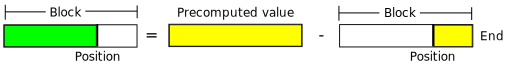
\includegraphics[width=\textwidth]{PrecomputePopcountBlock.pdf}
\figureEnd



\subsubsection{Page-aligning the Blocks}
Translation Lookaside Buffer misses are expensive and to avoid those, we can try to reduce the number of pages we load.
Using the precomputed vector of ranks, we only need to load pages of the bitmap at the beginning and end of each node's bitmap, to compute the popcount binary rank directly on the bitmap, and only within one block at each end.
If the blocks are not aligned with the memory pages, then, even if the block size is less than a page, it might span more than one page and thus more than one page of memory must be loaded into the TLB.
More precisely, we might at most load $\lceil\frac{blockSize}{pageSize}\rceil +1$ pages to do the popcount binary rank computation at the beginning and end of each node.

If we page-align the blocks, and use block sizes divisible by the page size or that page is divisible by, the extra $+1$ will disappear, because a block can no longer span more pages than its size is a multiple of the page size.
This means we can ensure that at most $2 \cdot \lceil\frac{blockSize}{pageSize}\rceil$ memory pages of the bitmap are loaded for each node by page-aligning the blocks.



\subsection{Select Queries with Precomputed Ranks}
Select queries, although they don't return a rank value, can still utilize the precomputed rank values to skip much computation directly on the bitmap by iterating though them.
Partway in a select query, if the sum of the occurrences found so far and the rank value of the current block of the bitmap is more than the queried-for occurrence, we can add that rank value to our occurrences seen so far and skip ahead to the next block and perform the same test.
If the sum is less than the queried-for occurrence, we know we will find the occurrence in the current block and switch back to the previous method of select querying using popcount starting at this block.


\subsubsection{Edge Cases}
As with rank queries, there are edge cases at the beginning and end of each bitmap.
However, in this case, the edge case at the end is easily handled as the test of sum of rank and occurrence-so-far should fail, sending the algorithm into the block with the previous select query method, finding the occurrence with no problem and no specific handling of the edge case.
This is assuming the input occurrence parameter is valid, that is, at least that many occurrences of that character is in the original input string.

For the other case, at the beginning of the bitmap, we do almost exactly the same as in the case for the rank query.
In fact, we use a rank query to calculate the rank of the first part of the bitmap, using the trick of subtracting from the precomputed value if larger than half a block size, to figure out whether the occurrence is in the first part of the bitmap, and therefore whether we should skip it or not.

\paragraph{Using Rank Queries in Select Queries}~\\
We would like to analyse whether it is worth using a rank query to find out whether we should do a select query on the first part of the bitmap, as the rank query is purely extra work in the cases where the occurrence is in that part of the bitmap.

We will assume an equal number of occurrences in the string of each character in the alphabet, a uniform distribution of each character in the string, and an equal probability of each valid parameter for the select query.
A valid character parameter is one that exists in the input string and a valid occurrence parameter is an integer above 0 and below or equal to the number occurrences appearing in the input string.

The rank query is a computation of worst-case cost $\frac{blockSize}{2}$ because it will at most popcount half of the block, because we utilize the precomputed rank value when advantageous.
The popcount select query into the first partial block is an operation of word-case cost $blockSize$ because it can at most popcount the entire block.
So, in the worst case, when the sought-after occurrence is in the first partial block of the bitmap, $\frac{blockSize}{2}$ work is wasted, yet when the occurrence is elsewhere, $blockSize$ work is saved.
This means that the boundary between where using the rank query becomes a gain or a loss in performance is where the ratio between times the occurrence is to be found in and outside the first partial block of the bitmap is $\nicefrac{2}{3}$.
That is, when the occurrence is to be found outside the first partial block of the bitmap less than two-thirds of the time, using the rank query first to see if that partial block should be select queried is a gain in performance, when considering the worst-case query time for both queries.

Though, this is giving the select query a disadvantage in the analysis, as, even when the partial block is close to a block in size, it might terminate early if it found the sought-after occurrence of the character early in the partial block.

It is not entirely clear whether it is an advantage to use the binary rank call, or it would be better to use popcount BinarySelect on the first partial block at all times.
We will test this in section~\ref{sec:experimentPrecomputedBlocksRankInSelect}



\subsection{Extra Space Used}
Since each precomputed value cannot exceed the block size in value, assuming we don't use block sizes exceeding $2^{16} = 65536$ bits, or $\frac{2^{16}}{8} = 8192$ bytes, we can store them in 16-bit unsigned integers, called \texttt{unsigned short int} on our machines. Since the page size on our machines are 4096 bits, that we should not use a block size larger than $\frac{65536}{4096} = 16$ pages if we want to use 16-bit unsigned integers.

In Section[TODO:reference] we find that the optimal block size is 16384 bits, or 4 pages.

Assuming we then store the precomputed values as 16-bit unsigned short integers it will only consume an extra 16 bits per block of which there are $\frac{BitmapSize}{BlockSize}$.
This means, assuming 4 pages per block, an extra space consumption of
\[ \frac{16}{16384} = 0.0009765625 = 0.098\% \]
of the bitmaps.
Which is even less when considering the total space used including the nodes, and would be less for larger block sizes.

Using one giant bitmap instead of one for each node might also cause a reduction in memory usage from no longer having unused, yet stored, bits at the end of each bitmap.


\subsection{Experiments}
\subsubsection{Query Running Time for Bitmap with Precomputed Blocks for different Block Sizes}

\subsubsection{Using Rank Queries in Select Queries}
\label{sec:experimentPrecomputedBlocksRankInSelect}

\subsubsection{Memory Usage of Concatenated vs. Individual Bitmaps}

\section{Precomputed Cumulative Sum of Binary Ranks}
We have found that using precomputed rank values is a great improvement to the running time of both rank and select queries, though with a higher gain for rank queries.
It works so well, because it allows the algorithms to skip most of the bitmaps, only directly using at them near the position that was queried for in case of rank queries and near the sought-after occurrence in the case of select queries, and relying on the precomputed values for the rest of the bitmap.

It does still, however, need to iterate through the precomputed values.
Most of the time the algorithms are interested in the rank value at some position inside a bitmap, it is the rank from the beginning of the bitmap to the position, rarely just the rank of that particular block.
Therefore we might be able to save a number of instructions by not iterating through the precomputed values if the precomputed values were already this cumulative sum of rank values through the bitmap.

We will implement this based on UnalignedNaive and test the performance compared to the UnalignedNaive tree from Section~\ref{sec:queryRunTimePrecomputedBlockSizes} as we found that to be the fastest.

\subsection{Advantages of Cumulative Sum}
As previously mentioned, the rank and select query algorithms don't actually need the rank values of individual blocks, but rather the cumulative sum rank value from the beginning of the bitmap to some position.
If we instead implemented the precomputed values as being the cumulative sum of rank values of each block from the beginning of the bitmap up to and including the block corresponding to the precomputed value, we could save a lot of precomputed value lookups in the rank and select queries.

Calculating the cumulative rank sums during the construction will not require much more computation.
It could e.g. be done by a single sweep through the precomputed values vector after having computed the entire bitmap, adding each precomputed value to the next in the vector.

Rank queries will benefit from the precomputed values being cumulative sums because they can do a single lookup of the precomputed value corresponding to the block covering the queried-for position.
The need to calculate a rank using \texttt{popcount}ing within a single block and manual counting of bits within a single word remains unchanged.

Select queries will also likely be quicker.
Previously, the select query would iterate through the precomputed values and sum them up, looking for when it surpasses the sought-after occurrence, and then calculate the position within a single block using \texttt{popcount} and manual counting of bits within a single word.
Using cumulative precomputed rank values, the select query will be able to use binary search on the precomputed value vector to find the word wherein the occurrence is.
Using \texttt{popcount} within a block and manual counting within a word still remains unchanged.

\subsection{Disadvantages of Cumulative Sum}
The precomputed values are no longer limited in value size by the block size but rather the bitmap size, as the last value in the precomputed rank value vector could potentially become as large as the bitmap is long.
Storing the cumulative sums will then require more bytes per value and thus use more space in the end.
The bitmap size is limited by the input string length and so for our choice of input string with length $10^8$ each precomputed value must be able to store a value up to $10^8$.
It takes at least 28 bits to store $10^8$, because $2^{27} < 10^8 < 2^{28}$.
Because the value types supported by x86 and C++ must be byte (8-bit) aligned and use a number of bytes that is a power of 2, the smallest type we can use is the 4-byte type \texttt{unsigned int} capable of storing values up to $2^{32}$.
This means the vector, instead of holding 2-byte \texttt{unsigned short int}s, must hold \texttt{unsigned int}s, doubling the space required to store the precomputed values.
We will see in our experiments whether the difference in running time can make up for the increase in storage space required.


\subsection{Experiments}

\subsection{Build Time}

\subsubsection{Rank Queries}

\subsubsection{Select Queries}


\newgeometry{left=2cm,right=2cm, top=2cm, bottom=3cm}

\begin{figure}\tiny
\begin{subfigure}{0.48\textwidth}
\input{CumulativeSumBuildWalltime}
\caption{Wall Time of Building the Wavelet tree}
\label{fig:CumulativeSumBuildWalltime}
\end{subfigure}
\caption{Measurements on Building the UnalignedNaive and CumulativeSum wavelet trees}
\label{fig:CumulativeSumBuild}
\end{figure}


\begin{figure}\tiny

\begin{subfigure}{0.48\textwidth}
	\input{CumulativeSumRankWalltime}
	\caption{Wall Time of Rank queries}
	\label{fig:CumulativeSumRankWalltime}
\end{subfigure}
\hfill
\begin{subfigure}{0.48\textwidth}
	\input{CumulativeSumRankBranchMiss}
	\caption{Branch Misses of Rank queries}
	\label{fig:CumulativeSumRankBranchMiss}
\end{subfigure}

\begin{subfigure}{0.48\textwidth}
	\input{CumulativeSumRankBranchExe}
	\caption{Branches Executed in Rank queries}
	\label{fig:CumulativeSumRankBranchExe}
\end{subfigure}
\hfill
\begin{subfigure}{0.48\textwidth}
	\input{CumulativeSumRankBranchMissRate}
	\caption{Branch Misprediction Rate of Rank queries}
	\label{fig:CumulativeSumRankBranchMissRate}
\end{subfigure}

\caption{Measurements on Rank Queries on the UnalignedNaive and CumulativeSum Wavelet Trees. Part 1.}
\label{fig:CumulativeSumRank}
\end{figure}




\begin{figure}\tiny

\begin{subfigure}{0.48\textwidth}
	\input{CumulativeSumRankTLBMiss}
	\caption{TLB Misses of Rank queries}
	\label{fig:CumulativeSumRankTLBMiss}
\end{subfigure}
\hfill
\begin{subfigure}{0.48\textwidth}
	\input{CumulativeSumRankL1CM}
	\caption{Level 1 Cache Misses of Rank queries}
	\label{fig:CumulativeSumRankL1CM}
\end{subfigure}

\begin{subfigure}{0.48\textwidth}
	\input{CumulativeSumRankL2CM}
	\caption{Level 2 Cache Misses in Rank queries}
	\label{fig:CumulativeSumRankL2CM}
\end{subfigure}
\hfill
\begin{subfigure}{0.48\textwidth}
	\input{CumulativeSumRankL2CHits}
	\caption{Level 2 Cache Hits of Rank queries}
	\label{fig:CumulativeSumRankL2CHits}
\end{subfigure}

\begin{subfigure}{0.48\textwidth}
	\input{CumulativeSumRankL2CMRate}
	\caption{Level 2 Cache Miss Rate in Rank queries}
	\label{fig:CumulativeSumRankL2CMRate}
\end{subfigure}
\hfill
\begin{subfigure}{0.48\textwidth}
	\input{CumulativeSumRankL3CM}
	\caption{Level 3 Cache Misses Rate of Rank queries}
	\label{fig:CumulativeSumRankL3CM}
\end{subfigure}

\caption{Measurements on Rank Queries on the UnalignedNaive and CumulativeSum Wavelet Trees. Part 2.}
\label{fig:CumulativeSumRank}
\end{figure}




\clearpage




\begin{figure}\tiny

\begin{subfigure}{0.48\textwidth}
	\input{CumulativeSumSelectWalltime}
	\caption{Wall Time of Select queries}
	\label{fig:CumulativeSumSelectWalltime}
\end{subfigure}
\hfill
\begin{subfigure}{0.48\textwidth}
	\input{CumulativeSumSelectBranchMiss}
	\caption{Branch Misses of Select queries}
	\label{fig:CumulativeSumSelectBranchMiss}
\end{subfigure}

\begin{subfigure}{0.48\textwidth}
	% GNUPLOT: LaTeX picture with Postscript
\begingroup
  \makeatletter
  \providecommand\color[2][]{%
    \GenericError{(gnuplot) \space\space\space\@spaces}{%
      Package color not loaded in conjunction with
      terminal option `colourtext'%
    }{See the gnuplot documentation for explanation.%
    }{Either use 'blacktext' in gnuplot or load the package
      color.sty in LaTeX.}%
    \renewcommand\color[2][]{}%
  }%
  \providecommand\includegraphics[2][]{%
    \GenericError{(gnuplot) \space\space\space\@spaces}{%
      Package graphicx or graphics not loaded%
    }{See the gnuplot documentation for explanation.%
    }{The gnuplot epslatex terminal needs graphicx.sty or graphics.sty.}%
    \renewcommand\includegraphics[2][]{}%
  }%
  \providecommand\rotatebox[2]{#2}%
  \@ifundefined{ifGPcolor}{%
    \newif\ifGPcolor
    \GPcolortrue
  }{}%
  \@ifundefined{ifGPblacktext}{%
    \newif\ifGPblacktext
    \GPblacktexttrue
  }{}%
  % define a \g@addto@macro without @ in the name:
  \let\gplgaddtomacro\g@addto@macro
  % define empty templates for all commands taking text:
  \gdef\gplbacktext{}%
  \gdef\gplfronttext{}%
  \makeatother
  \ifGPblacktext
    % no textcolor at all
    \def\colorrgb#1{}%
    \def\colorgray#1{}%
  \else
    % gray or color?
    \ifGPcolor
      \def\colorrgb#1{\color[rgb]{#1}}%
      \def\colorgray#1{\color[gray]{#1}}%
      \expandafter\def\csname LTw\endcsname{\color{white}}%
      \expandafter\def\csname LTb\endcsname{\color{black}}%
      \expandafter\def\csname LTa\endcsname{\color{black}}%
      \expandafter\def\csname LT0\endcsname{\color[rgb]{1,0,0}}%
      \expandafter\def\csname LT1\endcsname{\color[rgb]{0,1,0}}%
      \expandafter\def\csname LT2\endcsname{\color[rgb]{0,0,1}}%
      \expandafter\def\csname LT3\endcsname{\color[rgb]{1,0,1}}%
      \expandafter\def\csname LT4\endcsname{\color[rgb]{0,1,1}}%
      \expandafter\def\csname LT5\endcsname{\color[rgb]{1,1,0}}%
      \expandafter\def\csname LT6\endcsname{\color[rgb]{0,0,0}}%
      \expandafter\def\csname LT7\endcsname{\color[rgb]{1,0.3,0}}%
      \expandafter\def\csname LT8\endcsname{\color[rgb]{0.5,0.5,0.5}}%
    \else
      % gray
      \def\colorrgb#1{\color{black}}%
      \def\colorgray#1{\color[gray]{#1}}%
      \expandafter\def\csname LTw\endcsname{\color{white}}%
      \expandafter\def\csname LTb\endcsname{\color{black}}%
      \expandafter\def\csname LTa\endcsname{\color{black}}%
      \expandafter\def\csname LT0\endcsname{\color{black}}%
      \expandafter\def\csname LT1\endcsname{\color{black}}%
      \expandafter\def\csname LT2\endcsname{\color{black}}%
      \expandafter\def\csname LT3\endcsname{\color{black}}%
      \expandafter\def\csname LT4\endcsname{\color{black}}%
      \expandafter\def\csname LT5\endcsname{\color{black}}%
      \expandafter\def\csname LT6\endcsname{\color{black}}%
      \expandafter\def\csname LT7\endcsname{\color{black}}%
      \expandafter\def\csname LT8\endcsname{\color{black}}%
    \fi
  \fi
  \setlength{\unitlength}{0.0500bp}%
  \begin{picture}(3024.00,3600.00)%
    \gplgaddtomacro\gplbacktext{%
      \csname LTb\endcsname%
      \put(871,156){\makebox(0,0)[r]{\strut{} 0}}%
      \put(871,594){\makebox(0,0)[r]{\strut{} 2e+06}}%
      \put(871,1033){\makebox(0,0)[r]{\strut{} 4e+06}}%
      \put(871,1471){\makebox(0,0)[r]{\strut{} 6e+06}}%
      \put(871,1909){\makebox(0,0)[r]{\strut{} 8e+06}}%
      \put(871,2347){\makebox(0,0)[r]{\strut{} 1e+07}}%
      \put(871,2786){\makebox(0,0)[r]{\strut{} 1.2e+07}}%
      \put(871,3224){\makebox(0,0)[r]{\strut{} 1.4e+07}}%
      \put(104,1799){\rotatebox{-270}{\makebox(0,0){\strut{}Branches Executed}}}%
    }%
    \gplgaddtomacro\gplfronttext{%
      \csname LTb\endcsname%
      \put(2180,3315){\makebox(0,0)[r]{\strut{}UnalignedNaive}}%
      \csname LTb\endcsname%
      \put(2180,3185){\makebox(0,0)[r]{\strut{}CumulativeSum}}%
      \csname LTb\endcsname%
      \put(2180,3055){\makebox(0,0)[r]{\strut{}CumSumBranchless}}%
    }%
    \gplbacktext
    \put(0,0){\includegraphics{CumulativeSumSelectBranchExe}}%
    \gplfronttext
  \end{picture}%
\endgroup

	\caption{Branches Executed in Select queries}
	\label{fig:CumulativeSumSelectBranchExe}
\end{subfigure}
\hfill
\begin{subfigure}{0.48\textwidth}
	\input{CumulativeSumSelectBranchMissRate}
	\caption{Branch Misprediction Rate of Select queries}
	\label{fig:CumulativeSumSelectBranchMissRate}
\end{subfigure}

\caption{Measurements on Select Queries on the UnalignedNaive and CumulativeSum and CumulativeSumBranchless Wavelet Trees. Part 1.}
\label{fig:CumulativeSumSelect}
\end{figure}



\begin{figure}\tiny

\begin{subfigure}{0.48\textwidth}
	\input{CumulativeSumSelectTLBMiss}
	\caption{TLB Misses of Select queries}
	\label{fig:CumulativeSumSelectTLBMiss}
\end{subfigure}
\hfill
\begin{subfigure}{0.48\textwidth}
	\input{CumulativeSumSelectL1CM}
	\caption{Level 1 Cache Misses of Select queries}
	\label{fig:CumulativeSumSelectL1CM}
\end{subfigure}

\begin{subfigure}{0.48\textwidth}
	\input{CumulativeSumSelectL2CM}
	\caption{Level 2 Cache Misses in Select queries}
	\label{fig:CumulativeSumSelectL2CM}
\end{subfigure}
\hfill
\begin{subfigure}{0.48\textwidth}
	\input{CumulativeSumSelectL2CHits}
	\caption{Level 2 Cache Hits of Select queries}
	\label{fig:CumulativeSumSelectL2CHits}
\end{subfigure}

\begin{subfigure}{0.48\textwidth}
	\input{CumulativeSumSelectL2CMRate}
	\caption{Level 2 Cache Miss Rate in Select queries}
	\label{fig:CumulativeSumSelectL2CMRate}
\end{subfigure}
\hfill
\begin{subfigure}{0.48\textwidth}
	\input{CumulativeSumSelectL3CM}
	\caption{Level 3 Cache Misses Rate of Select queries}
	\label{fig:CumulativeSumSelectL3CM}
\end{subfigure}

\caption{Measurements on Select Queries on the UnalignedNaive and CumulativeSum and CumulativeSumBranchless Wavelet Trees. Part 2.}
\label{fig:CumulativeSumSelect}
\end{figure}






\restoregeometry















\section{Cumulative Sum with Controlled Memory Layout and Skew}
\label{sec:memorylayout}
In this section, we describe our attempt to improve the query times for the wavelet tree by controlling the memory layout and skewing the tree.
Skewing the tree means that we force the it to be unbalanced with a bias to one side. 
Brodal et al.~\citeA{gerthSkewedBinarySearchTrees} showed that skewing a binary search tree could reduce the amount of cache misses and branch mispredictions considerately. Enough, in fact, to increase the speed of searching the tree manyfold, even though the skewing increased the depth of the tree structure.

To reduce cache misses by skewing the tree we must control the memory layout, because by skewing the tree to the right, we increase the likelihood of a traversal similar to a depth-first-search going down the right side first (DFSr). So we want to place the data in memory so that a DFSr traversal through the tree would result in sequential address accesses.
Allocating memory dynamically as we go might produce a similar layout and controlling the memory may not lead to increased performance, but it is the only way to ensure the memory layout is as we want it.

Skewing the tree has the disadvantage of increasing the height, or depth, of the tree.
J.~Nievergelt and E.~M. Reingold~\citeB{Nievergelt:1972:BST:800152.804906} defined the height for a skewed binary tree to be at most:
\[ h_{max} = \frac{\log(m+1)}{ \log\frac{1}{1-\alpha}} \;,\]
where $m$ is the total number of nodes in the tree, that is $2 \sigma - 1$ in our wavelet tree, and $\alpha = \frac{1}{\mathit{skew}}$ and \textit{skew} is the number that is divided by to skew our tree, see Section~\ref{sec:SkewingTheTree}.
Together this makes the height at most
\[ h_{max} = \frac{\log(2 \sigma)}{ \log\frac{\mathit{skew}}{\mathit{skew} - 1}}  \;.\]
Which, when the tree is balanced, so $\mathit{skew} = 2$, makes the height at most $h_{max} = \log \sigma + 1$ which agrees with our definition of the height $h = \lceil \log \sigma \rceil$.

Let us analyse the theoretical worst case running time of constructing and querying a balanced wavelet tree vs. a skewed wavelet tree.

Constructing a balanced wavelet tree takes  $O(n \cdot \log \sigma)$ time because the height of the tree is $\lceil \log \sigma \rceil$ and there are $n$ elements in each level.
When skewing the tree the height of the tree becomes as defined above and the construction time becomes $O(n \cdot h_{max})$.

The query time for rank on a balanced wavelet tree is $O(b \log \sigma)$ and for select $O(b \log \sigma + \log \frac{n}{b} \log \sigma)$.
In the skewed version of the tree the rank query time then becomes worst-case $O(b \cdot h_{max})$. The query time for select becomes $O(b \cdot h_{max} + \log \frac{n}{b} \cdot h_{max})$

\textbf{[TODO: memory analysis]}

From the theoretical analysis of construction time and query time of a skewed wavelet tree it is theoretically not an improvement to skew the tree.
Skewing the tree can however reduce branch mispredictions, as shown by Brodal et al.~\citeA[Abstract]{gerthSkewedBinarySearchTrees}.
It does so by giving the branch in the direction the tree is skewed a much higher probability of being the correct than the other, which enables the branch prediction unit to predict correctly more often. 
Skewing the tree can also reduce cache misses by increasing the probability that the next piece of memory the algorithm accesses is already loaded into a cacheline by the time it is accessed because of prefetching.

The algorithms for construction and queries in this implementation remain mostly the same as before in CumulativeSum, but with modifications to handle a controlled memory layout and a skew of the tree.

\subsection{Prefetching}
Prefetching is a feature of the CPU whereby it can fetch other parts of the memory into cachelines even though it was not requested yet, if it believes it will be requested soon, to avoid having the program waiting for this fetching.
In more advanced versions, it can even look at the access into memory of the running program and try to determine a pattern and prefetch memory according to this pattern.
Looking at the Intel Optimization Manual~\citeB{intel-optimization-manual} for our architecture\footnote{Our architecture is Ivy Bridge, but the optimization manual sections for Sandy Bridge holds true for Ivy Bridge as well, as stated in section 2.2.7 in~\citeB{intel-optimization-manual}.} we find that it has streaming prefetchers loading into L1, L2, and last level cache. The streaming prefetchers detect accesses to ascending or descending addresses and can prefetch up to 20 lines ahead or behind. 
Our architecture also has a prefetcher that can detect strides in memory access, as well as a “Next Page Prefetcher” that can load another memory page when detecting memory accesses near the page boundary~\footnote{See section 2.2.7 of~\citeB{intel-optimization-manual}}.


\subsection{Skewing The Tree}
\label{sec:SkewingTheTree}
Skewing the tree is done by changing the way we find which character in the alphabet to split on in each node's construction.
The split character is the last character in the alphabet of the left child node and to be able to skew the calculation we calculate it as
\[\mathit{SplitCharacter} = \left\lfloor \frac{\mathit{alphabetSize}-1}{\mathit{skew}} + \mathit{alphabetMin} \right\rfloor \]
where \textit{alphabetSize} is the size of the alphabet at this node, \textit{alphabetMin} is the first character in the alphabet at this node, and \textit{skew} is the skew parameter which is 2 for a balanced tree and higher for right-skewed trees. E.g. a \textit{skew} value of 4 skews the tree by 75\,\% to the right so that, in each node, 25\,\% of the alphabet is put into the left child node and 75\,\% is put into the right child node.
We only use integer values as characters, so the calculated split character is rounded down.


\subsection{Controlled Memory Layout}
We still want to support dynamic input and alphabet sizes without recompilation, so the nodes must be dynamically allocated on the heap.

The size of a node is known at compile time as it contains fixed-size pointers to the parent node and left and right child nodes, as well as a boolean to flag it as a leaf node and its bitmap as a vector, which internally stores a pointer to its backing array.
As such, the memory for the nodes is allocated by allocating an array and then instantiating the nodes into that array.
A reference to a pointer is passed into the array from parent to child nodes during construction, so they know where to allocate their child nodes.
The pointer points to the position of the last node in the array, and so before each instantiation of a new node, we increment the pointer so it points to free space, then place the new node there.

The memory layout of the bitmaps are not controlled, because skewing the tree will not help the prefetcher with regards to the bitmaps, except in a few specific cases, because of the way the bitmaps are used and the resulting access patterns.
The algorithms for rank and select stop querying each bitmap at some position inside the bitmap and then continue to the next bitmap in the next node.
Rank stops when it reaches the position the query was searching up to, given as a parameter.
Select stops when it has found the sought number of occurrences in the bitmap.
In both these cases the rest of the bitmap is not used and any such data the prefetcher has fetched would have been in vain.
The prefetcher cannot tell from the algorithms access pattern when it will jump ahead to the next bitmap, and every such jump will therefore give rise to a cache miss.
The problem is shown in Figure~\ref{fig:QueryPrefetchFigure}. The drawing assumes the bitmap is stored sequentially and the prefetcher prefetches the next cache line (colored green), but the algorithm stops at some position and skips ahead to the next bitmap. 
This makes it unable to utilize the prefetched data and will try to access memory that is not in the cache yet; a cache miss.
So regardless of where the bitmap that is accessed next is stored, following right after the first or elsewhere in memory, a cache miss will occur.

The exceptions to this are when either the entire bitmap is used for the query, that is, when the rank query is for the entire string, or the bitmap is small enough that the beginning of the next bitmap can fit within the same word.
The first case is not a common query in most use cases, and the second case is rare when the input string is much bigger than the alphabet, and would only happen near the leaf nodes.
Neither scenario happens often enough to warrant controlling the bitmap memory layouts.

\figureBegin

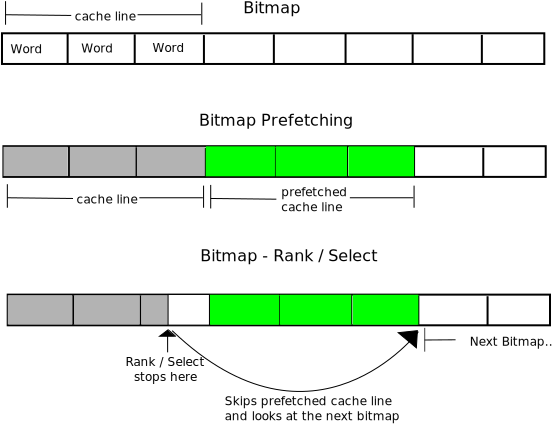
\includegraphics[width=\textwidth]{QueryPrefetchFigure.pdf}
\caption{How access patterns in a concatenated bitmap can defeat cache prefetching}
\label{fig:QueryPrefetchFigure}
\figureEnd



\subsection{Experiments}

\subsubsection{Queries when skewing the Wavelet Tree using uncontrolled and controlled memory layout}
In this experiment we want to test whether queries on a skewed tree using controlled memory layout is an improvement in running time.

\paragraph{Test Setup}~\\
The general setup is as described in Section~\ref{sec:ExpNotesGeneralSetup}.
The query parameters were chosen as described in Section~\ref{sec:choiceOfQueryParameters}.
The results can be seen in Figure~\ref{fig:NaiveRankSkewRunningTime} and Figure~\ref{fig:NaiveSelectSkewRunningTime}.
We skew the wavelet tree as described in Section~\ref{sec:SkewingTheTree}).

\paragraph{Results}~\\
\textbf{[TODO: complete rewrite with new graphs, results, etc. from this]}


\textbf{[TODO: new graphs]}

\iffalse
\newgeometry{left=2cm,right=2cm, top=2cm, bottom=3cm}

\begin{figure}\tiny
\begin{subfigure}{0.48\textwidth}
	\input{naiveRankSkewRunningTime}
	\caption{Wall Time}
	\label{fig:NaiveRankSkewRunningTime}
\end{subfigure}
\hfill
\begin{subfigure}{0.48\textwidth}
	% GNUPLOT: LaTeX picture with Postscript
\begingroup
  \makeatletter
  \providecommand\color[2][]{%
    \GenericError{(gnuplot) \space\space\space\@spaces}{%
      Package color not loaded in conjunction with
      terminal option `colourtext'%
    }{See the gnuplot documentation for explanation.%
    }{Either use 'blacktext' in gnuplot or load the package
      color.sty in LaTeX.}%
    \renewcommand\color[2][]{}%
  }%
  \providecommand\includegraphics[2][]{%
    \GenericError{(gnuplot) \space\space\space\@spaces}{%
      Package graphicx or graphics not loaded%
    }{See the gnuplot documentation for explanation.%
    }{The gnuplot epslatex terminal needs graphicx.sty or graphics.sty.}%
    \renewcommand\includegraphics[2][]{}%
  }%
  \providecommand\rotatebox[2]{#2}%
  \@ifundefined{ifGPcolor}{%
    \newif\ifGPcolor
    \GPcolortrue
  }{}%
  \@ifundefined{ifGPblacktext}{%
    \newif\ifGPblacktext
    \GPblacktexttrue
  }{}%
  % define a \g@addto@macro without @ in the name:
  \let\gplgaddtomacro\g@addto@macro
  % define empty templates for all commands taking text:
  \gdef\gplbacktext{}%
  \gdef\gplfronttext{}%
  \makeatother
  \ifGPblacktext
    % no textcolor at all
    \def\colorrgb#1{}%
    \def\colorgray#1{}%
  \else
    % gray or color?
    \ifGPcolor
      \def\colorrgb#1{\color[rgb]{#1}}%
      \def\colorgray#1{\color[gray]{#1}}%
      \expandafter\def\csname LTw\endcsname{\color{white}}%
      \expandafter\def\csname LTb\endcsname{\color{black}}%
      \expandafter\def\csname LTa\endcsname{\color{black}}%
      \expandafter\def\csname LT0\endcsname{\color[rgb]{1,0,0}}%
      \expandafter\def\csname LT1\endcsname{\color[rgb]{0,1,0}}%
      \expandafter\def\csname LT2\endcsname{\color[rgb]{0,0,1}}%
      \expandafter\def\csname LT3\endcsname{\color[rgb]{1,0,1}}%
      \expandafter\def\csname LT4\endcsname{\color[rgb]{0,1,1}}%
      \expandafter\def\csname LT5\endcsname{\color[rgb]{1,1,0}}%
      \expandafter\def\csname LT6\endcsname{\color[rgb]{0,0,0}}%
      \expandafter\def\csname LT7\endcsname{\color[rgb]{1,0.3,0}}%
      \expandafter\def\csname LT8\endcsname{\color[rgb]{0.5,0.5,0.5}}%
    \else
      % gray
      \def\colorrgb#1{\color{black}}%
      \def\colorgray#1{\color[gray]{#1}}%
      \expandafter\def\csname LTw\endcsname{\color{white}}%
      \expandafter\def\csname LTb\endcsname{\color{black}}%
      \expandafter\def\csname LTa\endcsname{\color{black}}%
      \expandafter\def\csname LT0\endcsname{\color{black}}%
      \expandafter\def\csname LT1\endcsname{\color{black}}%
      \expandafter\def\csname LT2\endcsname{\color{black}}%
      \expandafter\def\csname LT3\endcsname{\color{black}}%
      \expandafter\def\csname LT4\endcsname{\color{black}}%
      \expandafter\def\csname LT5\endcsname{\color{black}}%
      \expandafter\def\csname LT6\endcsname{\color{black}}%
      \expandafter\def\csname LT7\endcsname{\color{black}}%
      \expandafter\def\csname LT8\endcsname{\color{black}}%
    \fi
  \fi
  \setlength{\unitlength}{0.0500bp}%
  \begin{picture}(8062.00,4752.00)%
    \gplgaddtomacro\gplbacktext{%
      \csname LTb\endcsname%
      \put(1474,704){\makebox(0,0)[r]{\strut{} 0}}%
      \put(1474,1177){\makebox(0,0)[r]{\strut{} 2e-05}}%
      \put(1474,1650){\makebox(0,0)[r]{\strut{} 4e-05}}%
      \put(1474,2123){\makebox(0,0)[r]{\strut{} 6e-05}}%
      \put(1474,2596){\makebox(0,0)[r]{\strut{} 8e-05}}%
      \put(1474,3068){\makebox(0,0)[r]{\strut{} 0.0001}}%
      \put(1474,3541){\makebox(0,0)[r]{\strut{} 0.00012}}%
      \put(1474,4014){\makebox(0,0)[r]{\strut{} 0.00014}}%
      \put(1474,4487){\makebox(0,0)[r]{\strut{} 0.00016}}%
      \put(1606,484){\makebox(0,0){\strut{} 2}}%
      \put(2363,484){\makebox(0,0){\strut{} 2.5}}%
      \put(3121,484){\makebox(0,0){\strut{} 3}}%
      \put(3878,484){\makebox(0,0){\strut{} 3.5}}%
      \put(4636,484){\makebox(0,0){\strut{} 4}}%
      \put(5393,484){\makebox(0,0){\strut{} 4.5}}%
      \put(6150,484){\makebox(0,0){\strut{} 5}}%
      \put(6908,484){\makebox(0,0){\strut{} 5.5}}%
      \put(7665,484){\makebox(0,0){\strut{} 6}}%
      \put(176,2595){\rotatebox{-270}{\makebox(0,0){\strut{}Branch mis-prediction rate}}}%
      \put(4635,154){\makebox(0,0){\strut{}Skew}}%
    }%
    \gplgaddtomacro\gplfronttext{%
      \csname LTb\endcsname%
      \put(6678,1097){\makebox(0,0)[r]{\strut{}Naive}}%
      \csname LTb\endcsname%
      \put(6678,877){\makebox(0,0)[r]{\strut{}ControlledNodeMemory}}%
    }%
    \gplbacktext
    \put(0,0){\includegraphics{NaiveVsControlledNodeMemorySkewRankQuery_BMrate}}%
    \gplfronttext
  \end{picture}%
\endgroup

	\caption{Branch Misprediction Rate}
	\label{fig:NaiveVsControlledNodeMemorySkewRankQueryBMrate}
\end{subfigure}


\begin{subfigure}{0.48\textwidth}
	% GNUPLOT: LaTeX picture with Postscript
\begingroup
  \makeatletter
  \providecommand\color[2][]{%
    \GenericError{(gnuplot) \space\space\space\@spaces}{%
      Package color not loaded in conjunction with
      terminal option `colourtext'%
    }{See the gnuplot documentation for explanation.%
    }{Either use 'blacktext' in gnuplot or load the package
      color.sty in LaTeX.}%
    \renewcommand\color[2][]{}%
  }%
  \providecommand\includegraphics[2][]{%
    \GenericError{(gnuplot) \space\space\space\@spaces}{%
      Package graphicx or graphics not loaded%
    }{See the gnuplot documentation for explanation.%
    }{The gnuplot epslatex terminal needs graphicx.sty or graphics.sty.}%
    \renewcommand\includegraphics[2][]{}%
  }%
  \providecommand\rotatebox[2]{#2}%
  \@ifundefined{ifGPcolor}{%
    \newif\ifGPcolor
    \GPcolortrue
  }{}%
  \@ifundefined{ifGPblacktext}{%
    \newif\ifGPblacktext
    \GPblacktexttrue
  }{}%
  % define a \g@addto@macro without @ in the name:
  \let\gplgaddtomacro\g@addto@macro
  % define empty templates for all commands taking text:
  \gdef\gplbacktext{}%
  \gdef\gplfronttext{}%
  \makeatother
  \ifGPblacktext
    % no textcolor at all
    \def\colorrgb#1{}%
    \def\colorgray#1{}%
  \else
    % gray or color?
    \ifGPcolor
      \def\colorrgb#1{\color[rgb]{#1}}%
      \def\colorgray#1{\color[gray]{#1}}%
      \expandafter\def\csname LTw\endcsname{\color{white}}%
      \expandafter\def\csname LTb\endcsname{\color{black}}%
      \expandafter\def\csname LTa\endcsname{\color{black}}%
      \expandafter\def\csname LT0\endcsname{\color[rgb]{1,0,0}}%
      \expandafter\def\csname LT1\endcsname{\color[rgb]{0,1,0}}%
      \expandafter\def\csname LT2\endcsname{\color[rgb]{0,0,1}}%
      \expandafter\def\csname LT3\endcsname{\color[rgb]{1,0,1}}%
      \expandafter\def\csname LT4\endcsname{\color[rgb]{0,1,1}}%
      \expandafter\def\csname LT5\endcsname{\color[rgb]{1,1,0}}%
      \expandafter\def\csname LT6\endcsname{\color[rgb]{0,0,0}}%
      \expandafter\def\csname LT7\endcsname{\color[rgb]{1,0.3,0}}%
      \expandafter\def\csname LT8\endcsname{\color[rgb]{0.5,0.5,0.5}}%
    \else
      % gray
      \def\colorrgb#1{\color{black}}%
      \def\colorgray#1{\color[gray]{#1}}%
      \expandafter\def\csname LTw\endcsname{\color{white}}%
      \expandafter\def\csname LTb\endcsname{\color{black}}%
      \expandafter\def\csname LTa\endcsname{\color{black}}%
      \expandafter\def\csname LT0\endcsname{\color{black}}%
      \expandafter\def\csname LT1\endcsname{\color{black}}%
      \expandafter\def\csname LT2\endcsname{\color{black}}%
      \expandafter\def\csname LT3\endcsname{\color{black}}%
      \expandafter\def\csname LT4\endcsname{\color{black}}%
      \expandafter\def\csname LT5\endcsname{\color{black}}%
      \expandafter\def\csname LT6\endcsname{\color{black}}%
      \expandafter\def\csname LT7\endcsname{\color{black}}%
      \expandafter\def\csname LT8\endcsname{\color{black}}%
    \fi
  \fi
  \setlength{\unitlength}{0.0500bp}%
  \begin{picture}(7488.00,4464.00)%
    \gplgaddtomacro\gplbacktext{%
      \csname LTb\endcsname%
      \put(1474,704){\makebox(0,0)[r]{\strut{} 0}}%
      \put(1474,1109){\makebox(0,0)[r]{\strut{} 5e+07}}%
      \put(1474,1514){\makebox(0,0)[r]{\strut{} 1e+08}}%
      \put(1474,1919){\makebox(0,0)[r]{\strut{} 1.5e+08}}%
      \put(1474,2324){\makebox(0,0)[r]{\strut{} 2e+08}}%
      \put(1474,2729){\makebox(0,0)[r]{\strut{} 2.5e+08}}%
      \put(1474,3134){\makebox(0,0)[r]{\strut{} 3e+08}}%
      \put(1474,3539){\makebox(0,0)[r]{\strut{} 3.5e+08}}%
      \put(1606,484){\makebox(0,0){\strut{} 2}}%
      \put(2292,484){\makebox(0,0){\strut{} 2.5}}%
      \put(2977,484){\makebox(0,0){\strut{} 3}}%
      \put(3663,484){\makebox(0,0){\strut{} 3.5}}%
      \put(4349,484){\makebox(0,0){\strut{} 4}}%
      \put(5034,484){\makebox(0,0){\strut{} 4.5}}%
      \put(5720,484){\makebox(0,0){\strut{} 5}}%
      \put(6405,484){\makebox(0,0){\strut{} 5.5}}%
      \put(7091,484){\makebox(0,0){\strut{} 6}}%
      \put(176,2121){\rotatebox{-270}{\makebox(0,0){\strut{}Cache Misses}}}%
      \put(4348,154){\makebox(0,0){\strut{}Skew}}%
    }%
    \gplgaddtomacro\gplfronttext{%
      \csname LTb\endcsname%
      \put(6236,4291){\makebox(0,0)[r]{\strut{}Naive L1 $mr\hat{\sigma}=$0.015 $avg\hat{\sigma}=$0.01}}%
      \csname LTb\endcsname%
      \put(6236,4071){\makebox(0,0)[r]{\strut{}ControlledNodeMemory L1 $mr\hat{\sigma}=$0.034 $avg\hat{\sigma}=$0.01}}%
    }%
    \gplbacktext
    \put(0,0){\includegraphics{L1NaiveVsControlledNodeMemorySkewRankQueryCacheMisses}}%
    \gplfronttext
  \end{picture}%
\endgroup

	\caption{Level 1 Data Cache Misses}
	\label{fig:L1NaiveControlledNodeMemoryRankSkewCacheMisses}
\end{subfigure}
\hfill
\begin{subfigure}{0.48\textwidth}
 	% GNUPLOT: LaTeX picture with Postscript
\begingroup
  \makeatletter
  \providecommand\color[2][]{%
    \GenericError{(gnuplot) \space\space\space\@spaces}{%
      Package color not loaded in conjunction with
      terminal option `colourtext'%
    }{See the gnuplot documentation for explanation.%
    }{Either use 'blacktext' in gnuplot or load the package
      color.sty in LaTeX.}%
    \renewcommand\color[2][]{}%
  }%
  \providecommand\includegraphics[2][]{%
    \GenericError{(gnuplot) \space\space\space\@spaces}{%
      Package graphicx or graphics not loaded%
    }{See the gnuplot documentation for explanation.%
    }{The gnuplot epslatex terminal needs graphicx.sty or graphics.sty.}%
    \renewcommand\includegraphics[2][]{}%
  }%
  \providecommand\rotatebox[2]{#2}%
  \@ifundefined{ifGPcolor}{%
    \newif\ifGPcolor
    \GPcolortrue
  }{}%
  \@ifundefined{ifGPblacktext}{%
    \newif\ifGPblacktext
    \GPblacktexttrue
  }{}%
  % define a \g@addto@macro without @ in the name:
  \let\gplgaddtomacro\g@addto@macro
  % define empty templates for all commands taking text:
  \gdef\gplbacktext{}%
  \gdef\gplfronttext{}%
  \makeatother
  \ifGPblacktext
    % no textcolor at all
    \def\colorrgb#1{}%
    \def\colorgray#1{}%
  \else
    % gray or color?
    \ifGPcolor
      \def\colorrgb#1{\color[rgb]{#1}}%
      \def\colorgray#1{\color[gray]{#1}}%
      \expandafter\def\csname LTw\endcsname{\color{white}}%
      \expandafter\def\csname LTb\endcsname{\color{black}}%
      \expandafter\def\csname LTa\endcsname{\color{black}}%
      \expandafter\def\csname LT0\endcsname{\color[rgb]{1,0,0}}%
      \expandafter\def\csname LT1\endcsname{\color[rgb]{0,1,0}}%
      \expandafter\def\csname LT2\endcsname{\color[rgb]{0,0,1}}%
      \expandafter\def\csname LT3\endcsname{\color[rgb]{1,0,1}}%
      \expandafter\def\csname LT4\endcsname{\color[rgb]{0,1,1}}%
      \expandafter\def\csname LT5\endcsname{\color[rgb]{1,1,0}}%
      \expandafter\def\csname LT6\endcsname{\color[rgb]{0,0,0}}%
      \expandafter\def\csname LT7\endcsname{\color[rgb]{1,0.3,0}}%
      \expandafter\def\csname LT8\endcsname{\color[rgb]{0.5,0.5,0.5}}%
    \else
      % gray
      \def\colorrgb#1{\color{black}}%
      \def\colorgray#1{\color[gray]{#1}}%
      \expandafter\def\csname LTw\endcsname{\color{white}}%
      \expandafter\def\csname LTb\endcsname{\color{black}}%
      \expandafter\def\csname LTa\endcsname{\color{black}}%
      \expandafter\def\csname LT0\endcsname{\color{black}}%
      \expandafter\def\csname LT1\endcsname{\color{black}}%
      \expandafter\def\csname LT2\endcsname{\color{black}}%
      \expandafter\def\csname LT3\endcsname{\color{black}}%
      \expandafter\def\csname LT4\endcsname{\color{black}}%
      \expandafter\def\csname LT5\endcsname{\color{black}}%
      \expandafter\def\csname LT6\endcsname{\color{black}}%
      \expandafter\def\csname LT7\endcsname{\color{black}}%
      \expandafter\def\csname LT8\endcsname{\color{black}}%
    \fi
  \fi
  \setlength{\unitlength}{0.0500bp}%
  \begin{picture}(8062.00,4752.00)%
    \gplgaddtomacro\gplbacktext{%
      \csname LTb\endcsname%
      \put(1474,704){\makebox(0,0)[r]{\strut{} 0}}%
      \put(1474,1241){\makebox(0,0)[r]{\strut{} 500000}}%
      \put(1474,1777){\makebox(0,0)[r]{\strut{} 1e+06}}%
      \put(1474,2314){\makebox(0,0)[r]{\strut{} 1.5e+06}}%
      \put(1474,2850){\makebox(0,0)[r]{\strut{} 2e+06}}%
      \put(1474,3387){\makebox(0,0)[r]{\strut{} 2.5e+06}}%
      \put(1606,484){\makebox(0,0){\strut{} 2}}%
      \put(2363,484){\makebox(0,0){\strut{} 2.5}}%
      \put(3121,484){\makebox(0,0){\strut{} 3}}%
      \put(3878,484){\makebox(0,0){\strut{} 3.5}}%
      \put(4636,484){\makebox(0,0){\strut{} 4}}%
      \put(5393,484){\makebox(0,0){\strut{} 4.5}}%
      \put(6150,484){\makebox(0,0){\strut{} 5}}%
      \put(6908,484){\makebox(0,0){\strut{} 5.5}}%
      \put(7665,484){\makebox(0,0){\strut{} 6}}%
      \put(176,2045){\rotatebox{-270}{\makebox(0,0){\strut{}Cache Misses}}}%
      \put(4635,154){\makebox(0,0){\strut{}Skew}}%
    }%
    \gplgaddtomacro\gplfronttext{%
      \csname LTb\endcsname%
      \put(6810,4579){\makebox(0,0)[r]{\strut{}Naive L2 $mr\sigma=$14.203 $avg\sigma=$4.59}}%
      \csname LTb\endcsname%
      \put(6810,4359){\makebox(0,0)[r]{\strut{}Naive L3 $mr\sigma=$26.648 $avg\sigma=$12.87}}%
      \csname LTb\endcsname%
      \put(6810,4139){\makebox(0,0)[r]{\strut{}ControlledNodeMemory L2 $mr\sigma=$52.05 $avg\sigma=$19.79}}%
      \csname LTb\endcsname%
      \put(6810,3919){\makebox(0,0)[r]{\strut{}ControlledNodeMemory L3 $mr\sigma=$62.695 $avg\sigma=$32.46}}%
    }%
    \gplbacktext
    \put(0,0){\includegraphics{L2L3NaiveVsControlledNodeMemorySkewRankQueryCacheMisses}}%
    \gplfronttext
  \end{picture}%
\endgroup

	\caption{Level 2 Data and 3 Total Cache Misses}
	\label{fig:L2L3NaiveControlledNodeMemoryRankSkewCacheMisses}
\end{subfigure}

\begin{subfigure}{0.48\textwidth}
	% GNUPLOT: LaTeX picture with Postscript
\begingroup
  \makeatletter
  \providecommand\color[2][]{%
    \GenericError{(gnuplot) \space\space\space\@spaces}{%
      Package color not loaded in conjunction with
      terminal option `colourtext'%
    }{See the gnuplot documentation for explanation.%
    }{Either use 'blacktext' in gnuplot or load the package
      color.sty in LaTeX.}%
    \renewcommand\color[2][]{}%
  }%
  \providecommand\includegraphics[2][]{%
    \GenericError{(gnuplot) \space\space\space\@spaces}{%
      Package graphicx or graphics not loaded%
    }{See the gnuplot documentation for explanation.%
    }{The gnuplot epslatex terminal needs graphicx.sty or graphics.sty.}%
    \renewcommand\includegraphics[2][]{}%
  }%
  \providecommand\rotatebox[2]{#2}%
  \@ifundefined{ifGPcolor}{%
    \newif\ifGPcolor
    \GPcolortrue
  }{}%
  \@ifundefined{ifGPblacktext}{%
    \newif\ifGPblacktext
    \GPblacktexttrue
  }{}%
  % define a \g@addto@macro without @ in the name:
  \let\gplgaddtomacro\g@addto@macro
  % define empty templates for all commands taking text:
  \gdef\gplbacktext{}%
  \gdef\gplfronttext{}%
  \makeatother
  \ifGPblacktext
    % no textcolor at all
    \def\colorrgb#1{}%
    \def\colorgray#1{}%
  \else
    % gray or color?
    \ifGPcolor
      \def\colorrgb#1{\color[rgb]{#1}}%
      \def\colorgray#1{\color[gray]{#1}}%
      \expandafter\def\csname LTw\endcsname{\color{white}}%
      \expandafter\def\csname LTb\endcsname{\color{black}}%
      \expandafter\def\csname LTa\endcsname{\color{black}}%
      \expandafter\def\csname LT0\endcsname{\color[rgb]{1,0,0}}%
      \expandafter\def\csname LT1\endcsname{\color[rgb]{0,1,0}}%
      \expandafter\def\csname LT2\endcsname{\color[rgb]{0,0,1}}%
      \expandafter\def\csname LT3\endcsname{\color[rgb]{1,0,1}}%
      \expandafter\def\csname LT4\endcsname{\color[rgb]{0,1,1}}%
      \expandafter\def\csname LT5\endcsname{\color[rgb]{1,1,0}}%
      \expandafter\def\csname LT6\endcsname{\color[rgb]{0,0,0}}%
      \expandafter\def\csname LT7\endcsname{\color[rgb]{1,0.3,0}}%
      \expandafter\def\csname LT8\endcsname{\color[rgb]{0.5,0.5,0.5}}%
    \else
      % gray
      \def\colorrgb#1{\color{black}}%
      \def\colorgray#1{\color[gray]{#1}}%
      \expandafter\def\csname LTw\endcsname{\color{white}}%
      \expandafter\def\csname LTb\endcsname{\color{black}}%
      \expandafter\def\csname LTa\endcsname{\color{black}}%
      \expandafter\def\csname LT0\endcsname{\color{black}}%
      \expandafter\def\csname LT1\endcsname{\color{black}}%
      \expandafter\def\csname LT2\endcsname{\color{black}}%
      \expandafter\def\csname LT3\endcsname{\color{black}}%
      \expandafter\def\csname LT4\endcsname{\color{black}}%
      \expandafter\def\csname LT5\endcsname{\color{black}}%
      \expandafter\def\csname LT6\endcsname{\color{black}}%
      \expandafter\def\csname LT7\endcsname{\color{black}}%
      \expandafter\def\csname LT8\endcsname{\color{black}}%
    \fi
  \fi
  \setlength{\unitlength}{0.0500bp}%
  \begin{picture}(7488.00,4752.00)%
    \gplgaddtomacro\gplbacktext{%
      \csname LTb\endcsname%
      \put(1078,704){\makebox(0,0)[r]{\strut{} 0}}%
      \put(1078,1094){\makebox(0,0)[r]{\strut{} 0.01}}%
      \put(1078,1485){\makebox(0,0)[r]{\strut{} 0.02}}%
      \put(1078,1875){\makebox(0,0)[r]{\strut{} 0.03}}%
      \put(1078,2266){\makebox(0,0)[r]{\strut{} 0.04}}%
      \put(1078,2656){\makebox(0,0)[r]{\strut{} 0.05}}%
      \put(1078,3046){\makebox(0,0)[r]{\strut{} 0.06}}%
      \put(1078,3437){\makebox(0,0)[r]{\strut{} 0.07}}%
      \put(1078,3827){\makebox(0,0)[r]{\strut{} 0.08}}%
      \put(1210,484){\makebox(0,0){\strut{} 2}}%
      \put(1945,484){\makebox(0,0){\strut{} 2.5}}%
      \put(2680,484){\makebox(0,0){\strut{} 3}}%
      \put(3415,484){\makebox(0,0){\strut{} 3.5}}%
      \put(4151,484){\makebox(0,0){\strut{} 4}}%
      \put(4886,484){\makebox(0,0){\strut{} 4.5}}%
      \put(5621,484){\makebox(0,0){\strut{} 5}}%
      \put(6356,484){\makebox(0,0){\strut{} 5.5}}%
      \put(7091,484){\makebox(0,0){\strut{} 6}}%
      \put(176,2265){\rotatebox{-270}{\makebox(0,0){\strut{}L2 Cache miss rate}}}%
      \put(4150,154){\makebox(0,0){\strut{}Skew}}%
    }%
    \gplgaddtomacro\gplfronttext{%
      \csname LTb\endcsname%
      \put(6236,4579){\makebox(0,0)[r]{\strut{}Naive $mr\hat{\sigma}=$14.395 $avg\hat{\sigma}=$4.57}}%
      \csname LTb\endcsname%
      \put(6236,4359){\makebox(0,0)[r]{\strut{}ControlledNodeMemory $mr\hat{\sigma}=$55.041 $avg\hat{\sigma}=$20.23}}%
    }%
    \gplbacktext
    \put(0,0){\includegraphics{NaiveVsControlledNodeMemorySkewRankQuery_L2_DCMrate}}%
    \gplfronttext
  \end{picture}%
\endgroup

	\caption{Level 2 Data Cache Miss Rate}
	\label{fig:NaiveVsControlledNodeMemorySkewRankQuery_L2_DCMrate}
\end{subfigure}
\hfill
\begin{subfigure}{0.48\textwidth}
	% GNUPLOT: LaTeX picture with Postscript
\begingroup
  \makeatletter
  \providecommand\color[2][]{%
    \GenericError{(gnuplot) \space\space\space\@spaces}{%
      Package color not loaded in conjunction with
      terminal option `colourtext'%
    }{See the gnuplot documentation for explanation.%
    }{Either use 'blacktext' in gnuplot or load the package
      color.sty in LaTeX.}%
    \renewcommand\color[2][]{}%
  }%
  \providecommand\includegraphics[2][]{%
    \GenericError{(gnuplot) \space\space\space\@spaces}{%
      Package graphicx or graphics not loaded%
    }{See the gnuplot documentation for explanation.%
    }{The gnuplot epslatex terminal needs graphicx.sty or graphics.sty.}%
    \renewcommand\includegraphics[2][]{}%
  }%
  \providecommand\rotatebox[2]{#2}%
  \@ifundefined{ifGPcolor}{%
    \newif\ifGPcolor
    \GPcolortrue
  }{}%
  \@ifundefined{ifGPblacktext}{%
    \newif\ifGPblacktext
    \GPblacktexttrue
  }{}%
  % define a \g@addto@macro without @ in the name:
  \let\gplgaddtomacro\g@addto@macro
  % define empty templates for all commands taking text:
  \gdef\gplbacktext{}%
  \gdef\gplfronttext{}%
  \makeatother
  \ifGPblacktext
    % no textcolor at all
    \def\colorrgb#1{}%
    \def\colorgray#1{}%
  \else
    % gray or color?
    \ifGPcolor
      \def\colorrgb#1{\color[rgb]{#1}}%
      \def\colorgray#1{\color[gray]{#1}}%
      \expandafter\def\csname LTw\endcsname{\color{white}}%
      \expandafter\def\csname LTb\endcsname{\color{black}}%
      \expandafter\def\csname LTa\endcsname{\color{black}}%
      \expandafter\def\csname LT0\endcsname{\color[rgb]{1,0,0}}%
      \expandafter\def\csname LT1\endcsname{\color[rgb]{0,1,0}}%
      \expandafter\def\csname LT2\endcsname{\color[rgb]{0,0,1}}%
      \expandafter\def\csname LT3\endcsname{\color[rgb]{1,0,1}}%
      \expandafter\def\csname LT4\endcsname{\color[rgb]{0,1,1}}%
      \expandafter\def\csname LT5\endcsname{\color[rgb]{1,1,0}}%
      \expandafter\def\csname LT6\endcsname{\color[rgb]{0,0,0}}%
      \expandafter\def\csname LT7\endcsname{\color[rgb]{1,0.3,0}}%
      \expandafter\def\csname LT8\endcsname{\color[rgb]{0.5,0.5,0.5}}%
    \else
      % gray
      \def\colorrgb#1{\color{black}}%
      \def\colorgray#1{\color[gray]{#1}}%
      \expandafter\def\csname LTw\endcsname{\color{white}}%
      \expandafter\def\csname LTb\endcsname{\color{black}}%
      \expandafter\def\csname LTa\endcsname{\color{black}}%
      \expandafter\def\csname LT0\endcsname{\color{black}}%
      \expandafter\def\csname LT1\endcsname{\color{black}}%
      \expandafter\def\csname LT2\endcsname{\color{black}}%
      \expandafter\def\csname LT3\endcsname{\color{black}}%
      \expandafter\def\csname LT4\endcsname{\color{black}}%
      \expandafter\def\csname LT5\endcsname{\color{black}}%
      \expandafter\def\csname LT6\endcsname{\color{black}}%
      \expandafter\def\csname LT7\endcsname{\color{black}}%
      \expandafter\def\csname LT8\endcsname{\color{black}}%
    \fi
  \fi
  \setlength{\unitlength}{0.0500bp}%
  \begin{picture}(7488.00,4752.00)%
    \gplgaddtomacro\gplbacktext{%
      \csname LTb\endcsname%
      \put(1342,704){\makebox(0,0)[r]{\strut{} 0}}%
      \put(1342,1094){\makebox(0,0)[r]{\strut{} 20000}}%
      \put(1342,1485){\makebox(0,0)[r]{\strut{} 40000}}%
      \put(1342,1875){\makebox(0,0)[r]{\strut{} 60000}}%
      \put(1342,2266){\makebox(0,0)[r]{\strut{} 80000}}%
      \put(1342,2656){\makebox(0,0)[r]{\strut{} 100000}}%
      \put(1342,3046){\makebox(0,0)[r]{\strut{} 120000}}%
      \put(1342,3437){\makebox(0,0)[r]{\strut{} 140000}}%
      \put(1342,3827){\makebox(0,0)[r]{\strut{} 160000}}%
      \put(1474,484){\makebox(0,0){\strut{} 2}}%
      \put(2176,484){\makebox(0,0){\strut{} 2.5}}%
      \put(2878,484){\makebox(0,0){\strut{} 3}}%
      \put(3580,484){\makebox(0,0){\strut{} 3.5}}%
      \put(4283,484){\makebox(0,0){\strut{} 4}}%
      \put(4985,484){\makebox(0,0){\strut{} 4.5}}%
      \put(5687,484){\makebox(0,0){\strut{} 5}}%
      \put(6389,484){\makebox(0,0){\strut{} 5.5}}%
      \put(7091,484){\makebox(0,0){\strut{} 6}}%
      \put(176,2265){\rotatebox{-270}{\makebox(0,0){\strut{}TLB}}}%
      \put(4282,154){\makebox(0,0){\strut{}Skew}}%
    }%
    \gplgaddtomacro\gplfronttext{%
      \csname LTb\endcsname%
      \put(6236,4579){\makebox(0,0)[r]{\strut{}Naive $mr\hat{\sigma}=$77.255 $avg\hat{\sigma}=$38.8}}%
      \csname LTb\endcsname%
      \put(6236,4359){\makebox(0,0)[r]{\strut{}ControlledNodeMemory $mr\hat{\sigma}=$106.361 $avg\hat{\sigma}=$38.66}}%
    }%
    \gplbacktext
    \put(0,0){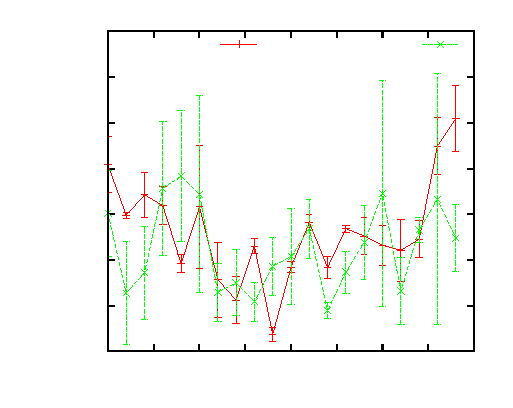
\includegraphics{NaiveVsControlledNodeMemorySkewRankQueryTLB}}%
    \gplfronttext
  \end{picture}%
\endgroup

	\caption{TLB Misses}
	\label{fig:NaiveVsControlledNodeMemorySkewRankQueryTLB}
\end{subfigure}

\caption{Various measurements for Rank queries on SimpleNaive and ControlledMemory wavelet trees with various skew.}
\label{fig:NaiveVsControlledNodeMemorySkewRankQuery}

\end{figure}



\begin{figure}\tiny
\begin{subfigure}{0.48\textwidth}
	% GNUPLOT: LaTeX picture with Postscript
\begingroup
  \makeatletter
  \providecommand\color[2][]{%
    \GenericError{(gnuplot) \space\space\space\@spaces}{%
      Package color not loaded in conjunction with
      terminal option `colourtext'%
    }{See the gnuplot documentation for explanation.%
    }{Either use 'blacktext' in gnuplot or load the package
      color.sty in LaTeX.}%
    \renewcommand\color[2][]{}%
  }%
  \providecommand\includegraphics[2][]{%
    \GenericError{(gnuplot) \space\space\space\@spaces}{%
      Package graphicx or graphics not loaded%
    }{See the gnuplot documentation for explanation.%
    }{The gnuplot epslatex terminal needs graphicx.sty or graphics.sty.}%
    \renewcommand\includegraphics[2][]{}%
  }%
  \providecommand\rotatebox[2]{#2}%
  \@ifundefined{ifGPcolor}{%
    \newif\ifGPcolor
    \GPcolortrue
  }{}%
  \@ifundefined{ifGPblacktext}{%
    \newif\ifGPblacktext
    \GPblacktexttrue
  }{}%
  % define a \g@addto@macro without @ in the name:
  \let\gplgaddtomacro\g@addto@macro
  % define empty templates for all commands taking text:
  \gdef\gplbacktext{}%
  \gdef\gplfronttext{}%
  \makeatother
  \ifGPblacktext
    % no textcolor at all
    \def\colorrgb#1{}%
    \def\colorgray#1{}%
  \else
    % gray or color?
    \ifGPcolor
      \def\colorrgb#1{\color[rgb]{#1}}%
      \def\colorgray#1{\color[gray]{#1}}%
      \expandafter\def\csname LTw\endcsname{\color{white}}%
      \expandafter\def\csname LTb\endcsname{\color{black}}%
      \expandafter\def\csname LTa\endcsname{\color{black}}%
      \expandafter\def\csname LT0\endcsname{\color[rgb]{1,0,0}}%
      \expandafter\def\csname LT1\endcsname{\color[rgb]{0,1,0}}%
      \expandafter\def\csname LT2\endcsname{\color[rgb]{0,0,1}}%
      \expandafter\def\csname LT3\endcsname{\color[rgb]{1,0,1}}%
      \expandafter\def\csname LT4\endcsname{\color[rgb]{0,1,1}}%
      \expandafter\def\csname LT5\endcsname{\color[rgb]{1,1,0}}%
      \expandafter\def\csname LT6\endcsname{\color[rgb]{0,0,0}}%
      \expandafter\def\csname LT7\endcsname{\color[rgb]{1,0.3,0}}%
      \expandafter\def\csname LT8\endcsname{\color[rgb]{0.5,0.5,0.5}}%
    \else
      % gray
      \def\colorrgb#1{\color{black}}%
      \def\colorgray#1{\color[gray]{#1}}%
      \expandafter\def\csname LTw\endcsname{\color{white}}%
      \expandafter\def\csname LTb\endcsname{\color{black}}%
      \expandafter\def\csname LTa\endcsname{\color{black}}%
      \expandafter\def\csname LT0\endcsname{\color{black}}%
      \expandafter\def\csname LT1\endcsname{\color{black}}%
      \expandafter\def\csname LT2\endcsname{\color{black}}%
      \expandafter\def\csname LT3\endcsname{\color{black}}%
      \expandafter\def\csname LT4\endcsname{\color{black}}%
      \expandafter\def\csname LT5\endcsname{\color{black}}%
      \expandafter\def\csname LT6\endcsname{\color{black}}%
      \expandafter\def\csname LT7\endcsname{\color{black}}%
      \expandafter\def\csname LT8\endcsname{\color{black}}%
    \fi
  \fi
  \setlength{\unitlength}{0.0500bp}%
  \begin{picture}(4608.00,3600.00)%
    \gplgaddtomacro\gplbacktext{%
      \csname LTb\endcsname%
      \put(588,384){\makebox(0,0)[r]{\strut{} 0}}%
      \put(588,1082){\makebox(0,0)[r]{\strut{} 0.05}}%
      \put(588,1780){\makebox(0,0)[r]{\strut{} 0.1}}%
      \put(588,2478){\makebox(0,0)[r]{\strut{} 0.15}}%
      \put(588,3176){\makebox(0,0)[r]{\strut{} 0.2}}%
      \put(660,264){\makebox(0,0){\strut{} 2}}%
      \put(1126,264){\makebox(0,0){\strut{} 2.5}}%
      \put(1593,264){\makebox(0,0){\strut{} 3}}%
      \put(2059,264){\makebox(0,0){\strut{} 3.5}}%
      \put(2526,264){\makebox(0,0){\strut{} 4}}%
      \put(2992,264){\makebox(0,0){\strut{} 4.5}}%
      \put(3458,264){\makebox(0,0){\strut{} 5}}%
      \put(3925,264){\makebox(0,0){\strut{} 5.5}}%
      \put(4391,264){\makebox(0,0){\strut{} 6}}%
      \put(96,1919){\rotatebox{-270}{\makebox(0,0){\strut{}Wall Time (sec)}}}%
      \put(2525,84){\makebox(0,0){\strut{}Skew}}%
    }%
    \gplgaddtomacro\gplfronttext{%
      \csname LTb\endcsname%
      \put(1884,3332){\makebox(0,0)[r]{\strut{}NaiveInteger}}%
      \csname LTb\endcsname%
      \put(3531,3332){\makebox(0,0)[r]{\strut{}ControlledMemory}}%
    }%
    \gplbacktext
    \put(0,0){\includegraphics{naiveSelectSkewRunningTime}}%
    \gplfronttext
  \end{picture}%
\endgroup

	\caption{Wall Time}
	\label{fig:NaiveSelectSkewRunningTime}
\end{subfigure}
\hfill
\begin{subfigure}{0.48\textwidth}
	% GNUPLOT: LaTeX picture with Postscript
\begingroup
  \makeatletter
  \providecommand\color[2][]{%
    \GenericError{(gnuplot) \space\space\space\@spaces}{%
      Package color not loaded in conjunction with
      terminal option `colourtext'%
    }{See the gnuplot documentation for explanation.%
    }{Either use 'blacktext' in gnuplot or load the package
      color.sty in LaTeX.}%
    \renewcommand\color[2][]{}%
  }%
  \providecommand\includegraphics[2][]{%
    \GenericError{(gnuplot) \space\space\space\@spaces}{%
      Package graphicx or graphics not loaded%
    }{See the gnuplot documentation for explanation.%
    }{The gnuplot epslatex terminal needs graphicx.sty or graphics.sty.}%
    \renewcommand\includegraphics[2][]{}%
  }%
  \providecommand\rotatebox[2]{#2}%
  \@ifundefined{ifGPcolor}{%
    \newif\ifGPcolor
    \GPcolortrue
  }{}%
  \@ifundefined{ifGPblacktext}{%
    \newif\ifGPblacktext
    \GPblacktexttrue
  }{}%
  % define a \g@addto@macro without @ in the name:
  \let\gplgaddtomacro\g@addto@macro
  % define empty templates for all commands taking text:
  \gdef\gplbacktext{}%
  \gdef\gplfronttext{}%
  \makeatother
  \ifGPblacktext
    % no textcolor at all
    \def\colorrgb#1{}%
    \def\colorgray#1{}%
  \else
    % gray or color?
    \ifGPcolor
      \def\colorrgb#1{\color[rgb]{#1}}%
      \def\colorgray#1{\color[gray]{#1}}%
      \expandafter\def\csname LTw\endcsname{\color{white}}%
      \expandafter\def\csname LTb\endcsname{\color{black}}%
      \expandafter\def\csname LTa\endcsname{\color{black}}%
      \expandafter\def\csname LT0\endcsname{\color[rgb]{1,0,0}}%
      \expandafter\def\csname LT1\endcsname{\color[rgb]{0,1,0}}%
      \expandafter\def\csname LT2\endcsname{\color[rgb]{0,0,1}}%
      \expandafter\def\csname LT3\endcsname{\color[rgb]{1,0,1}}%
      \expandafter\def\csname LT4\endcsname{\color[rgb]{0,1,1}}%
      \expandafter\def\csname LT5\endcsname{\color[rgb]{1,1,0}}%
      \expandafter\def\csname LT6\endcsname{\color[rgb]{0,0,0}}%
      \expandafter\def\csname LT7\endcsname{\color[rgb]{1,0.3,0}}%
      \expandafter\def\csname LT8\endcsname{\color[rgb]{0.5,0.5,0.5}}%
    \else
      % gray
      \def\colorrgb#1{\color{black}}%
      \def\colorgray#1{\color[gray]{#1}}%
      \expandafter\def\csname LTw\endcsname{\color{white}}%
      \expandafter\def\csname LTb\endcsname{\color{black}}%
      \expandafter\def\csname LTa\endcsname{\color{black}}%
      \expandafter\def\csname LT0\endcsname{\color{black}}%
      \expandafter\def\csname LT1\endcsname{\color{black}}%
      \expandafter\def\csname LT2\endcsname{\color{black}}%
      \expandafter\def\csname LT3\endcsname{\color{black}}%
      \expandafter\def\csname LT4\endcsname{\color{black}}%
      \expandafter\def\csname LT5\endcsname{\color{black}}%
      \expandafter\def\csname LT6\endcsname{\color{black}}%
      \expandafter\def\csname LT7\endcsname{\color{black}}%
      \expandafter\def\csname LT8\endcsname{\color{black}}%
    \fi
  \fi
  \setlength{\unitlength}{0.0500bp}%
  \begin{picture}(7488.00,4464.00)%
    \gplgaddtomacro\gplbacktext{%
      \csname LTb\endcsname%
      \put(1474,704){\makebox(0,0)[r]{\strut{} 0}}%
      \put(1474,1058){\makebox(0,0)[r]{\strut{} 2e-05}}%
      \put(1474,1413){\makebox(0,0)[r]{\strut{} 4e-05}}%
      \put(1474,1767){\makebox(0,0)[r]{\strut{} 6e-05}}%
      \put(1474,2122){\makebox(0,0)[r]{\strut{} 8e-05}}%
      \put(1474,2476){\makebox(0,0)[r]{\strut{} 0.0001}}%
      \put(1474,2830){\makebox(0,0)[r]{\strut{} 0.00012}}%
      \put(1474,3185){\makebox(0,0)[r]{\strut{} 0.00014}}%
      \put(1474,3539){\makebox(0,0)[r]{\strut{} 0.00016}}%
      \put(1606,484){\makebox(0,0){\strut{} 2}}%
      \put(2292,484){\makebox(0,0){\strut{} 2.5}}%
      \put(2977,484){\makebox(0,0){\strut{} 3}}%
      \put(3663,484){\makebox(0,0){\strut{} 3.5}}%
      \put(4349,484){\makebox(0,0){\strut{} 4}}%
      \put(5034,484){\makebox(0,0){\strut{} 4.5}}%
      \put(5720,484){\makebox(0,0){\strut{} 5}}%
      \put(6405,484){\makebox(0,0){\strut{} 5.5}}%
      \put(7091,484){\makebox(0,0){\strut{} 6}}%
      \put(176,2121){\rotatebox{-270}{\makebox(0,0){\strut{}Branch Misprediction Rate}}}%
      \put(4348,154){\makebox(0,0){\strut{}Skew}}%
    }%
    \gplgaddtomacro\gplfronttext{%
      \csname LTb\endcsname%
      \put(6236,4291){\makebox(0,0)[r]{\strut{}Naive $mr\hat{\sigma}=$0.407 $avg\hat{\sigma}=$0.15}}%
      \csname LTb\endcsname%
      \put(6236,4071){\makebox(0,0)[r]{\strut{}ControlledNodeMemory $mr\hat{\sigma}=$0.333 $avg\hat{\sigma}=$0.16}}%
    }%
    \gplbacktext
    \put(0,0){\includegraphics{NaiveVsControlledNodeMemorySkewSelectQuery_BMrate}}%
    \gplfronttext
  \end{picture}%
\endgroup

	\caption{Branch Misprediction Rate}
	\label{fig:NaiveVsControlledNodeMemorySkewSelectQueryBMrate}
\end{subfigure}

\begin{subfigure}{0.48\textwidth}
	\input{L1NaiveVsControlledNodeMemorySkewSelectQueryCacheMisses}
	\caption{Level 1 Data Cache Misses}
	\label{fig:L1NaiveControlledNodeMemorySelectSkewCacheMisses}
\end{subfigure}
\hfill
\begin{subfigure}{0.48\textwidth}
 	% GNUPLOT: LaTeX picture with Postscript
\begingroup
  \makeatletter
  \providecommand\color[2][]{%
    \GenericError{(gnuplot) \space\space\space\@spaces}{%
      Package color not loaded in conjunction with
      terminal option `colourtext'%
    }{See the gnuplot documentation for explanation.%
    }{Either use 'blacktext' in gnuplot or load the package
      color.sty in LaTeX.}%
    \renewcommand\color[2][]{}%
  }%
  \providecommand\includegraphics[2][]{%
    \GenericError{(gnuplot) \space\space\space\@spaces}{%
      Package graphicx or graphics not loaded%
    }{See the gnuplot documentation for explanation.%
    }{The gnuplot epslatex terminal needs graphicx.sty or graphics.sty.}%
    \renewcommand\includegraphics[2][]{}%
  }%
  \providecommand\rotatebox[2]{#2}%
  \@ifundefined{ifGPcolor}{%
    \newif\ifGPcolor
    \GPcolortrue
  }{}%
  \@ifundefined{ifGPblacktext}{%
    \newif\ifGPblacktext
    \GPblacktexttrue
  }{}%
  % define a \g@addto@macro without @ in the name:
  \let\gplgaddtomacro\g@addto@macro
  % define empty templates for all commands taking text:
  \gdef\gplbacktext{}%
  \gdef\gplfronttext{}%
  \makeatother
  \ifGPblacktext
    % no textcolor at all
    \def\colorrgb#1{}%
    \def\colorgray#1{}%
  \else
    % gray or color?
    \ifGPcolor
      \def\colorrgb#1{\color[rgb]{#1}}%
      \def\colorgray#1{\color[gray]{#1}}%
      \expandafter\def\csname LTw\endcsname{\color{white}}%
      \expandafter\def\csname LTb\endcsname{\color{black}}%
      \expandafter\def\csname LTa\endcsname{\color{black}}%
      \expandafter\def\csname LT0\endcsname{\color[rgb]{1,0,0}}%
      \expandafter\def\csname LT1\endcsname{\color[rgb]{0,1,0}}%
      \expandafter\def\csname LT2\endcsname{\color[rgb]{0,0,1}}%
      \expandafter\def\csname LT3\endcsname{\color[rgb]{1,0,1}}%
      \expandafter\def\csname LT4\endcsname{\color[rgb]{0,1,1}}%
      \expandafter\def\csname LT5\endcsname{\color[rgb]{1,1,0}}%
      \expandafter\def\csname LT6\endcsname{\color[rgb]{0,0,0}}%
      \expandafter\def\csname LT7\endcsname{\color[rgb]{1,0.3,0}}%
      \expandafter\def\csname LT8\endcsname{\color[rgb]{0.5,0.5,0.5}}%
    \else
      % gray
      \def\colorrgb#1{\color{black}}%
      \def\colorgray#1{\color[gray]{#1}}%
      \expandafter\def\csname LTw\endcsname{\color{white}}%
      \expandafter\def\csname LTb\endcsname{\color{black}}%
      \expandafter\def\csname LTa\endcsname{\color{black}}%
      \expandafter\def\csname LT0\endcsname{\color{black}}%
      \expandafter\def\csname LT1\endcsname{\color{black}}%
      \expandafter\def\csname LT2\endcsname{\color{black}}%
      \expandafter\def\csname LT3\endcsname{\color{black}}%
      \expandafter\def\csname LT4\endcsname{\color{black}}%
      \expandafter\def\csname LT5\endcsname{\color{black}}%
      \expandafter\def\csname LT6\endcsname{\color{black}}%
      \expandafter\def\csname LT7\endcsname{\color{black}}%
      \expandafter\def\csname LT8\endcsname{\color{black}}%
    \fi
  \fi
  \setlength{\unitlength}{0.0500bp}%
  \begin{picture}(7488.00,4464.00)%
    \gplgaddtomacro\gplbacktext{%
      \csname LTb\endcsname%
      \put(1474,704){\makebox(0,0)[r]{\strut{} 0}}%
      \put(1474,1003){\makebox(0,0)[r]{\strut{} 2e+06}}%
      \put(1474,1303){\makebox(0,0)[r]{\strut{} 4e+06}}%
      \put(1474,1602){\makebox(0,0)[r]{\strut{} 6e+06}}%
      \put(1474,1902){\makebox(0,0)[r]{\strut{} 8e+06}}%
      \put(1474,2201){\makebox(0,0)[r]{\strut{} 1e+07}}%
      \put(1474,2500){\makebox(0,0)[r]{\strut{} 1.2e+07}}%
      \put(1474,2800){\makebox(0,0)[r]{\strut{} 1.4e+07}}%
      \put(1474,3099){\makebox(0,0)[r]{\strut{} 1.6e+07}}%
      \put(1606,484){\makebox(0,0){\strut{} 2}}%
      \put(2292,484){\makebox(0,0){\strut{} 2.5}}%
      \put(2977,484){\makebox(0,0){\strut{} 3}}%
      \put(3663,484){\makebox(0,0){\strut{} 3.5}}%
      \put(4349,484){\makebox(0,0){\strut{} 4}}%
      \put(5034,484){\makebox(0,0){\strut{} 4.5}}%
      \put(5720,484){\makebox(0,0){\strut{} 5}}%
      \put(6405,484){\makebox(0,0){\strut{} 5.5}}%
      \put(7091,484){\makebox(0,0){\strut{} 6}}%
      \put(176,1901){\rotatebox{-270}{\makebox(0,0){\strut{}Cache Misses}}}%
      \put(4348,154){\makebox(0,0){\strut{}Skew}}%
    }%
    \gplgaddtomacro\gplfronttext{%
      \csname LTb\endcsname%
      \put(6236,4291){\makebox(0,0)[r]{\strut{}Naive L2 $mr\hat{\sigma}=$8.869 $avg\hat{\sigma}=$3.47}}%
      \csname LTb\endcsname%
      \put(6236,4071){\makebox(0,0)[r]{\strut{}Naive L3 $mr\hat{\sigma}=$6.579 $avg\hat{\sigma}=$3.91}}%
      \csname LTb\endcsname%
      \put(6236,3851){\makebox(0,0)[r]{\strut{}ControlledNodeMemory L2 $mr\hat{\sigma}=$6.829 $avg\hat{\sigma}=$3.8}}%
      \csname LTb\endcsname%
      \put(6236,3631){\makebox(0,0)[r]{\strut{}ControlledNodeMemory L3 $mr\hat{\sigma}=$5.604 $avg\hat{\sigma}=$3.95}}%
    }%
    \gplbacktext
    \put(0,0){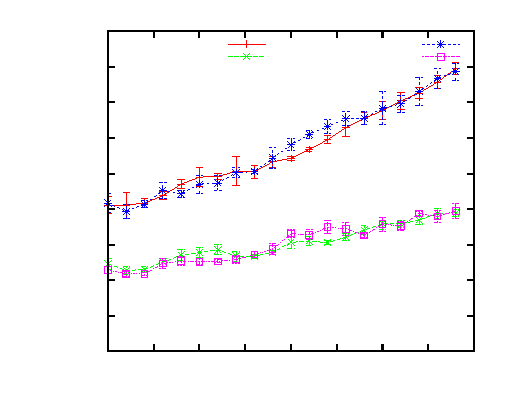
\includegraphics{L2L3NaiveVsControlledNodeMemorySkewSelectQueryCacheMisses}}%
    \gplfronttext
  \end{picture}%
\endgroup

	\caption{Level 2 Data and 3 Total Cache Misses}
	\label{fig:L2L3NaiveControlledNodeMemorySelectSkewCacheMisses}
\end{subfigure}

\begin{subfigure}{0.48\textwidth}
	% GNUPLOT: LaTeX picture with Postscript
\begingroup
  \makeatletter
  \providecommand\color[2][]{%
    \GenericError{(gnuplot) \space\space\space\@spaces}{%
      Package color not loaded in conjunction with
      terminal option `colourtext'%
    }{See the gnuplot documentation for explanation.%
    }{Either use 'blacktext' in gnuplot or load the package
      color.sty in LaTeX.}%
    \renewcommand\color[2][]{}%
  }%
  \providecommand\includegraphics[2][]{%
    \GenericError{(gnuplot) \space\space\space\@spaces}{%
      Package graphicx or graphics not loaded%
    }{See the gnuplot documentation for explanation.%
    }{The gnuplot epslatex terminal needs graphicx.sty or graphics.sty.}%
    \renewcommand\includegraphics[2][]{}%
  }%
  \providecommand\rotatebox[2]{#2}%
  \@ifundefined{ifGPcolor}{%
    \newif\ifGPcolor
    \GPcolortrue
  }{}%
  \@ifundefined{ifGPblacktext}{%
    \newif\ifGPblacktext
    \GPblacktexttrue
  }{}%
  % define a \g@addto@macro without @ in the name:
  \let\gplgaddtomacro\g@addto@macro
  % define empty templates for all commands taking text:
  \gdef\gplbacktext{}%
  \gdef\gplfronttext{}%
  \makeatother
  \ifGPblacktext
    % no textcolor at all
    \def\colorrgb#1{}%
    \def\colorgray#1{}%
  \else
    % gray or color?
    \ifGPcolor
      \def\colorrgb#1{\color[rgb]{#1}}%
      \def\colorgray#1{\color[gray]{#1}}%
      \expandafter\def\csname LTw\endcsname{\color{white}}%
      \expandafter\def\csname LTb\endcsname{\color{black}}%
      \expandafter\def\csname LTa\endcsname{\color{black}}%
      \expandafter\def\csname LT0\endcsname{\color[rgb]{1,0,0}}%
      \expandafter\def\csname LT1\endcsname{\color[rgb]{0,1,0}}%
      \expandafter\def\csname LT2\endcsname{\color[rgb]{0,0,1}}%
      \expandafter\def\csname LT3\endcsname{\color[rgb]{1,0,1}}%
      \expandafter\def\csname LT4\endcsname{\color[rgb]{0,1,1}}%
      \expandafter\def\csname LT5\endcsname{\color[rgb]{1,1,0}}%
      \expandafter\def\csname LT6\endcsname{\color[rgb]{0,0,0}}%
      \expandafter\def\csname LT7\endcsname{\color[rgb]{1,0.3,0}}%
      \expandafter\def\csname LT8\endcsname{\color[rgb]{0.5,0.5,0.5}}%
    \else
      % gray
      \def\colorrgb#1{\color{black}}%
      \def\colorgray#1{\color[gray]{#1}}%
      \expandafter\def\csname LTw\endcsname{\color{white}}%
      \expandafter\def\csname LTb\endcsname{\color{black}}%
      \expandafter\def\csname LTa\endcsname{\color{black}}%
      \expandafter\def\csname LT0\endcsname{\color{black}}%
      \expandafter\def\csname LT1\endcsname{\color{black}}%
      \expandafter\def\csname LT2\endcsname{\color{black}}%
      \expandafter\def\csname LT3\endcsname{\color{black}}%
      \expandafter\def\csname LT4\endcsname{\color{black}}%
      \expandafter\def\csname LT5\endcsname{\color{black}}%
      \expandafter\def\csname LT6\endcsname{\color{black}}%
      \expandafter\def\csname LT7\endcsname{\color{black}}%
      \expandafter\def\csname LT8\endcsname{\color{black}}%
    \fi
  \fi
  \setlength{\unitlength}{0.0500bp}%
  \begin{picture}(4608.00,3600.00)%
    \gplgaddtomacro\gplbacktext{%
      \csname LTb\endcsname%
      \put(588,384){\makebox(0,0)[r]{\strut{} 0}}%
      \put(588,768){\makebox(0,0)[r]{\strut{} 0.01}}%
      \put(588,1152){\makebox(0,0)[r]{\strut{} 0.02}}%
      \put(588,1536){\makebox(0,0)[r]{\strut{} 0.03}}%
      \put(588,1920){\makebox(0,0)[r]{\strut{} 0.04}}%
      \put(588,2303){\makebox(0,0)[r]{\strut{} 0.05}}%
      \put(588,2687){\makebox(0,0)[r]{\strut{} 0.06}}%
      \put(588,3071){\makebox(0,0)[r]{\strut{} 0.07}}%
      \put(588,3455){\makebox(0,0)[r]{\strut{} 0.08}}%
      \put(660,264){\makebox(0,0){\strut{} 2}}%
      \put(1126,264){\makebox(0,0){\strut{} 2.5}}%
      \put(1593,264){\makebox(0,0){\strut{} 3}}%
      \put(2059,264){\makebox(0,0){\strut{} 3.5}}%
      \put(2526,264){\makebox(0,0){\strut{} 4}}%
      \put(2992,264){\makebox(0,0){\strut{} 4.5}}%
      \put(3458,264){\makebox(0,0){\strut{} 5}}%
      \put(3925,264){\makebox(0,0){\strut{} 5.5}}%
      \put(4391,264){\makebox(0,0){\strut{} 6}}%
      \put(96,1919){\rotatebox{-270}{\makebox(0,0){\strut{}L2 Cache miss rate}}}%
      \put(2525,84){\makebox(0,0){\strut{}Skew}}%
    }%
    \gplgaddtomacro\gplfronttext{%
      \csname LTb\endcsname%
      \put(1884,3332){\makebox(0,0)[r]{\strut{}SimpleNaive}}%
      \csname LTb\endcsname%
      \put(3531,3332){\makebox(0,0)[r]{\strut{}ControlledMemory}}%
    }%
    \gplbacktext
    \put(0,0){\includegraphics{NaiveVsControlledNodeMemorySkewSelectQuery_L2_DCMrate}}%
    \gplfronttext
  \end{picture}%
\endgroup

	\caption{Level 2 Data Cache Miss Rate}
	\label{fig:NaiveVsControlledNodeMemorySkewSelectQuery_L2_DCMrate}
\end{subfigure}
\hfill
\begin{subfigure}{0.48\textwidth}
	\input{NaiveVsControlledNodeMemorySkewSelectQueryTLB}
	\caption{TLB Misses}
	\label{fig:NaiveVsControlledNodeMemorySkewSelectQueryTLB}
\end{subfigure}

\caption{Various measurements for Select queries on SimpleNaive and ControlledMemory wavelet trees with various skew.}
\label{fig:NaiveVsControlledNodeMemorySkewSelectQuery}

\end{figure}


\restoregeometry
\fi

\newpage
\clearpage
\part{Conclusion}

\section{Conclusion}
In this Thesis we have performed a short survey on the applications of wavelet trees and described in more detail for some of the uses ... \textbf{[TODO: something something]}

We have implemented and tested rank and select queries for a number of 

\section{Future Work}
We have many ideas for future work on practical implementation and optimization on wavelet trees.

\subsection{vEB Memory Layout}
\label{sec:futurework_vebmemorylayout}
We tried a right-side depth-first memory layout in Section~\ref{sec:memorylayout} when we tried to skew the tree.
Without trying to skew the tree, other memory layouts might still be able to improve the performance of the wavelet tree.
Brodal et al.~\citeA{gerthSkewedBinarySearchTrees} tested several memory layouts for their skewed binary search tree and found that the blocked memory layout based on van Emde Boas Trees performed best for all skew values.
It could be interesting to try a van Embe Boas memory layout for a balanced wavelet tree to see if it could improve the query performance.

\subsection{Skew}
In Section~\ref{sec:memorylayout} we tried skewing the tree to reduce cache misses and branch mispredictions and found that it was no improvement, in part because the wavelet tree spends most of the time in the rank or select queries calculating binary rank or select on the bitmaps.
With our optimizations from later sections, we have reduced the amount of time spent calculating binary rank and select, and it is possible that skewing the tree might have a beneficial effect after having applied our other optimizations.

\subsection{$d$-ary}
Our wavelet trees are all binary which means their height is the base-2 logarithm of the alphabet size.
With a $d$-ary tree the height would be reduced to base $d$ logarithm of the alphabet size.
This could improve access, rank, and select query performance significantly as their traversal down or up the tree would be significantly shortened.

A disadvantage of a $d$-ary wavelet tree is that each bitmap must encode $\log_2(d)$ bits of information for each character in the string, to signify which of the subtrees each character belongs to.
This, in turn, makes using the native \texttt{popcount} cpu instruction impossible, perhaps unless some clever bitshifting and \texttt{XOR}ring could be applied to avoid manually counting sets of bits.
On the other hand, using the stored precomputed values means only few sets of bits would have to be counted and perhaps the benefit from a lower tree will outweigh the loss from not using \texttt{popcount}.

\subsubsection{SIMD}
When constructing or traversing a $d$-ary wavelet tree, finding which of 4 or more subtrees to either pass a character too or traverse into requires comparing the character with more than just one split character.
To improve the performance of this multi-way comparison, SIMD instructions might be employed with success.


\subsection{Parallelization}
To expand on the potential improvement from using SIMD instructions when constructing and traversing $d$-ary wavelet trees, some amount of parallelization of the algorithms might improve the performance even further.
\subsubsection{On GPU}
If parallelization proves to be an improvement, implementing them on the GPU e.g. using CUDA could be a massive improvement as modern GPUs have several hundred cores and if well-utilized can surpass the power of a modern CPU.




\newgeometry{left=2cm,right=2cm, top=2cm, bottom=3cm}
\begin{appendices}


\section{Precomputed rank block sizes: larger range}
\begin{figure}[h!]\tiny
\begin{subfigure}{0.48\textwidth}
	% GNUPLOT: LaTeX picture with Postscript
\begingroup
  \makeatletter
  \providecommand\color[2][]{%
    \GenericError{(gnuplot) \space\space\space\@spaces}{%
      Package color not loaded in conjunction with
      terminal option `colourtext'%
    }{See the gnuplot documentation for explanation.%
    }{Either use 'blacktext' in gnuplot or load the package
      color.sty in LaTeX.}%
    \renewcommand\color[2][]{}%
  }%
  \providecommand\includegraphics[2][]{%
    \GenericError{(gnuplot) \space\space\space\@spaces}{%
      Package graphicx or graphics not loaded%
    }{See the gnuplot documentation for explanation.%
    }{The gnuplot epslatex terminal needs graphicx.sty or graphics.sty.}%
    \renewcommand\includegraphics[2][]{}%
  }%
  \providecommand\rotatebox[2]{#2}%
  \@ifundefined{ifGPcolor}{%
    \newif\ifGPcolor
    \GPcolortrue
  }{}%
  \@ifundefined{ifGPblacktext}{%
    \newif\ifGPblacktext
    \GPblacktexttrue
  }{}%
  % define a \g@addto@macro without @ in the name:
  \let\gplgaddtomacro\g@addto@macro
  % define empty templates for all commands taking text:
  \gdef\gplbacktext{}%
  \gdef\gplfronttext{}%
  \makeatother
  \ifGPblacktext
    % no textcolor at all
    \def\colorrgb#1{}%
    \def\colorgray#1{}%
  \else
    % gray or color?
    \ifGPcolor
      \def\colorrgb#1{\color[rgb]{#1}}%
      \def\colorgray#1{\color[gray]{#1}}%
      \expandafter\def\csname LTw\endcsname{\color{white}}%
      \expandafter\def\csname LTb\endcsname{\color{black}}%
      \expandafter\def\csname LTa\endcsname{\color{black}}%
      \expandafter\def\csname LT0\endcsname{\color[rgb]{1,0,0}}%
      \expandafter\def\csname LT1\endcsname{\color[rgb]{0,1,0}}%
      \expandafter\def\csname LT2\endcsname{\color[rgb]{0,0,1}}%
      \expandafter\def\csname LT3\endcsname{\color[rgb]{1,0,1}}%
      \expandafter\def\csname LT4\endcsname{\color[rgb]{0,1,1}}%
      \expandafter\def\csname LT5\endcsname{\color[rgb]{1,1,0}}%
      \expandafter\def\csname LT6\endcsname{\color[rgb]{0,0,0}}%
      \expandafter\def\csname LT7\endcsname{\color[rgb]{1,0.3,0}}%
      \expandafter\def\csname LT8\endcsname{\color[rgb]{0.5,0.5,0.5}}%
    \else
      % gray
      \def\colorrgb#1{\color{black}}%
      \def\colorgray#1{\color[gray]{#1}}%
      \expandafter\def\csname LTw\endcsname{\color{white}}%
      \expandafter\def\csname LTb\endcsname{\color{black}}%
      \expandafter\def\csname LTa\endcsname{\color{black}}%
      \expandafter\def\csname LT0\endcsname{\color{black}}%
      \expandafter\def\csname LT1\endcsname{\color{black}}%
      \expandafter\def\csname LT2\endcsname{\color{black}}%
      \expandafter\def\csname LT3\endcsname{\color{black}}%
      \expandafter\def\csname LT4\endcsname{\color{black}}%
      \expandafter\def\csname LT5\endcsname{\color{black}}%
      \expandafter\def\csname LT6\endcsname{\color{black}}%
      \expandafter\def\csname LT7\endcsname{\color{black}}%
      \expandafter\def\csname LT8\endcsname{\color{black}}%
    \fi
  \fi
  \setlength{\unitlength}{0.0500bp}%
  \begin{picture}(4608.00,3600.00)%
    \gplgaddtomacro\gplbacktext{%
      \csname LTb\endcsname%
      \put(732,384){\makebox(0,0)[r]{\strut{} 1000}}%
      \put(732,1408){\makebox(0,0)[r]{\strut{} 10000}}%
      \put(732,2431){\makebox(0,0)[r]{\strut{} 100000}}%
      \put(732,3455){\makebox(0,0)[r]{\strut{} 1e+06}}%
      \put(804,264){\makebox(0,0){\strut{}$2^{6}$}}%
      \put(1316,264){\makebox(0,0){\strut{}$2^{8}$}}%
      \put(1829,264){\makebox(0,0){\strut{}$2^{10}$}}%
      \put(2341,264){\makebox(0,0){\strut{}$2^{12}$}}%
      \put(2854,264){\makebox(0,0){\strut{}$2^{14}$}}%
      \put(3366,264){\makebox(0,0){\strut{}$2^{16}$}}%
      \put(3879,264){\makebox(0,0){\strut{}$2^{18}$}}%
      \put(4391,264){\makebox(0,0){\strut{}$2^{20}$}}%
      \put(96,1919){\rotatebox{-270}{\makebox(0,0){\strut{}Wall Time ($\mu s$)}}}%
      \put(2597,84){\makebox(0,0){\strut{}Block Size (bits)}}%
    }%
    \gplgaddtomacro\gplfronttext{%
      \csname LTb\endcsname%
      \put(3824,3332){\makebox(0,0)[r]{\strut{}Naive}}%
      \csname LTb\endcsname%
      \put(3824,3212){\makebox(0,0)[r]{\strut{}Preallocated}}%
      \csname LTb\endcsname%
      \put(3824,3092){\makebox(0,0)[r]{\strut{}UnalignedNaive}}%
      \csname LTb\endcsname%
      \put(3824,2972){\makebox(0,0)[r]{\strut{}UnalignedPreallocated}}%
    }%
    \gplbacktext
    \put(0,0){\includegraphics{PrecomputedRankBlockSizeLarger_Rank_WallTime}}%
    \gplfronttext
  \end{picture}%
\endgroup

	\caption{Rank: Wall Time}
	\label{fig:PrecomputedRankBlockSize_Rank_WallTime}
\end{subfigure}
\hfill
\begin{subfigure}{0.48\textwidth}
	\input{PrecomputedRankBlockSizeLarger_Select_WallTime}
	\caption{Select: Wall Time}
	\label{fig:PrecomputedRankBlockSize_Select_WallTime}
\end{subfigure}
\caption{Running time for Rank queries in Wavelet Trees with Precomputed Rank Values for larger range of varying block sizes. A page size is $2^{15}$ bits.}
\end{figure}

\end{appendices}
\restoregeometry

\addcontentsline{toc}{section}{Primary Bibliography}
\bibliographystyleA{unsrtnat}
\bibliographyA{Report}
\addcontentsline{toc}{section}{Secondary Bibliography (not curriculum)}
\bibliographystyleB{unsrtnat}
\bibliographyB{Report}

\end{document}
